%-  LaTeX source file

%-  performance.tex ~~
%
%   This is the fourth section of the paper.
%
%                                                   ~~ last updated 05 Dec 2018

%Availability note: code supporting this section is available at
%\url{https://github.com/ATLAS-Titan/moab-data}. 

%\subsection{Scaling PanDA on Titan}
%\label{subsec:scaling}

%See Figure ~\ref{fig:throughput-all} \ldots
%% For two-column wide figures use
%\begin{figure*}
%% Use the relevant command to insert your figure file.
%% For example, with the graphicx package use
%  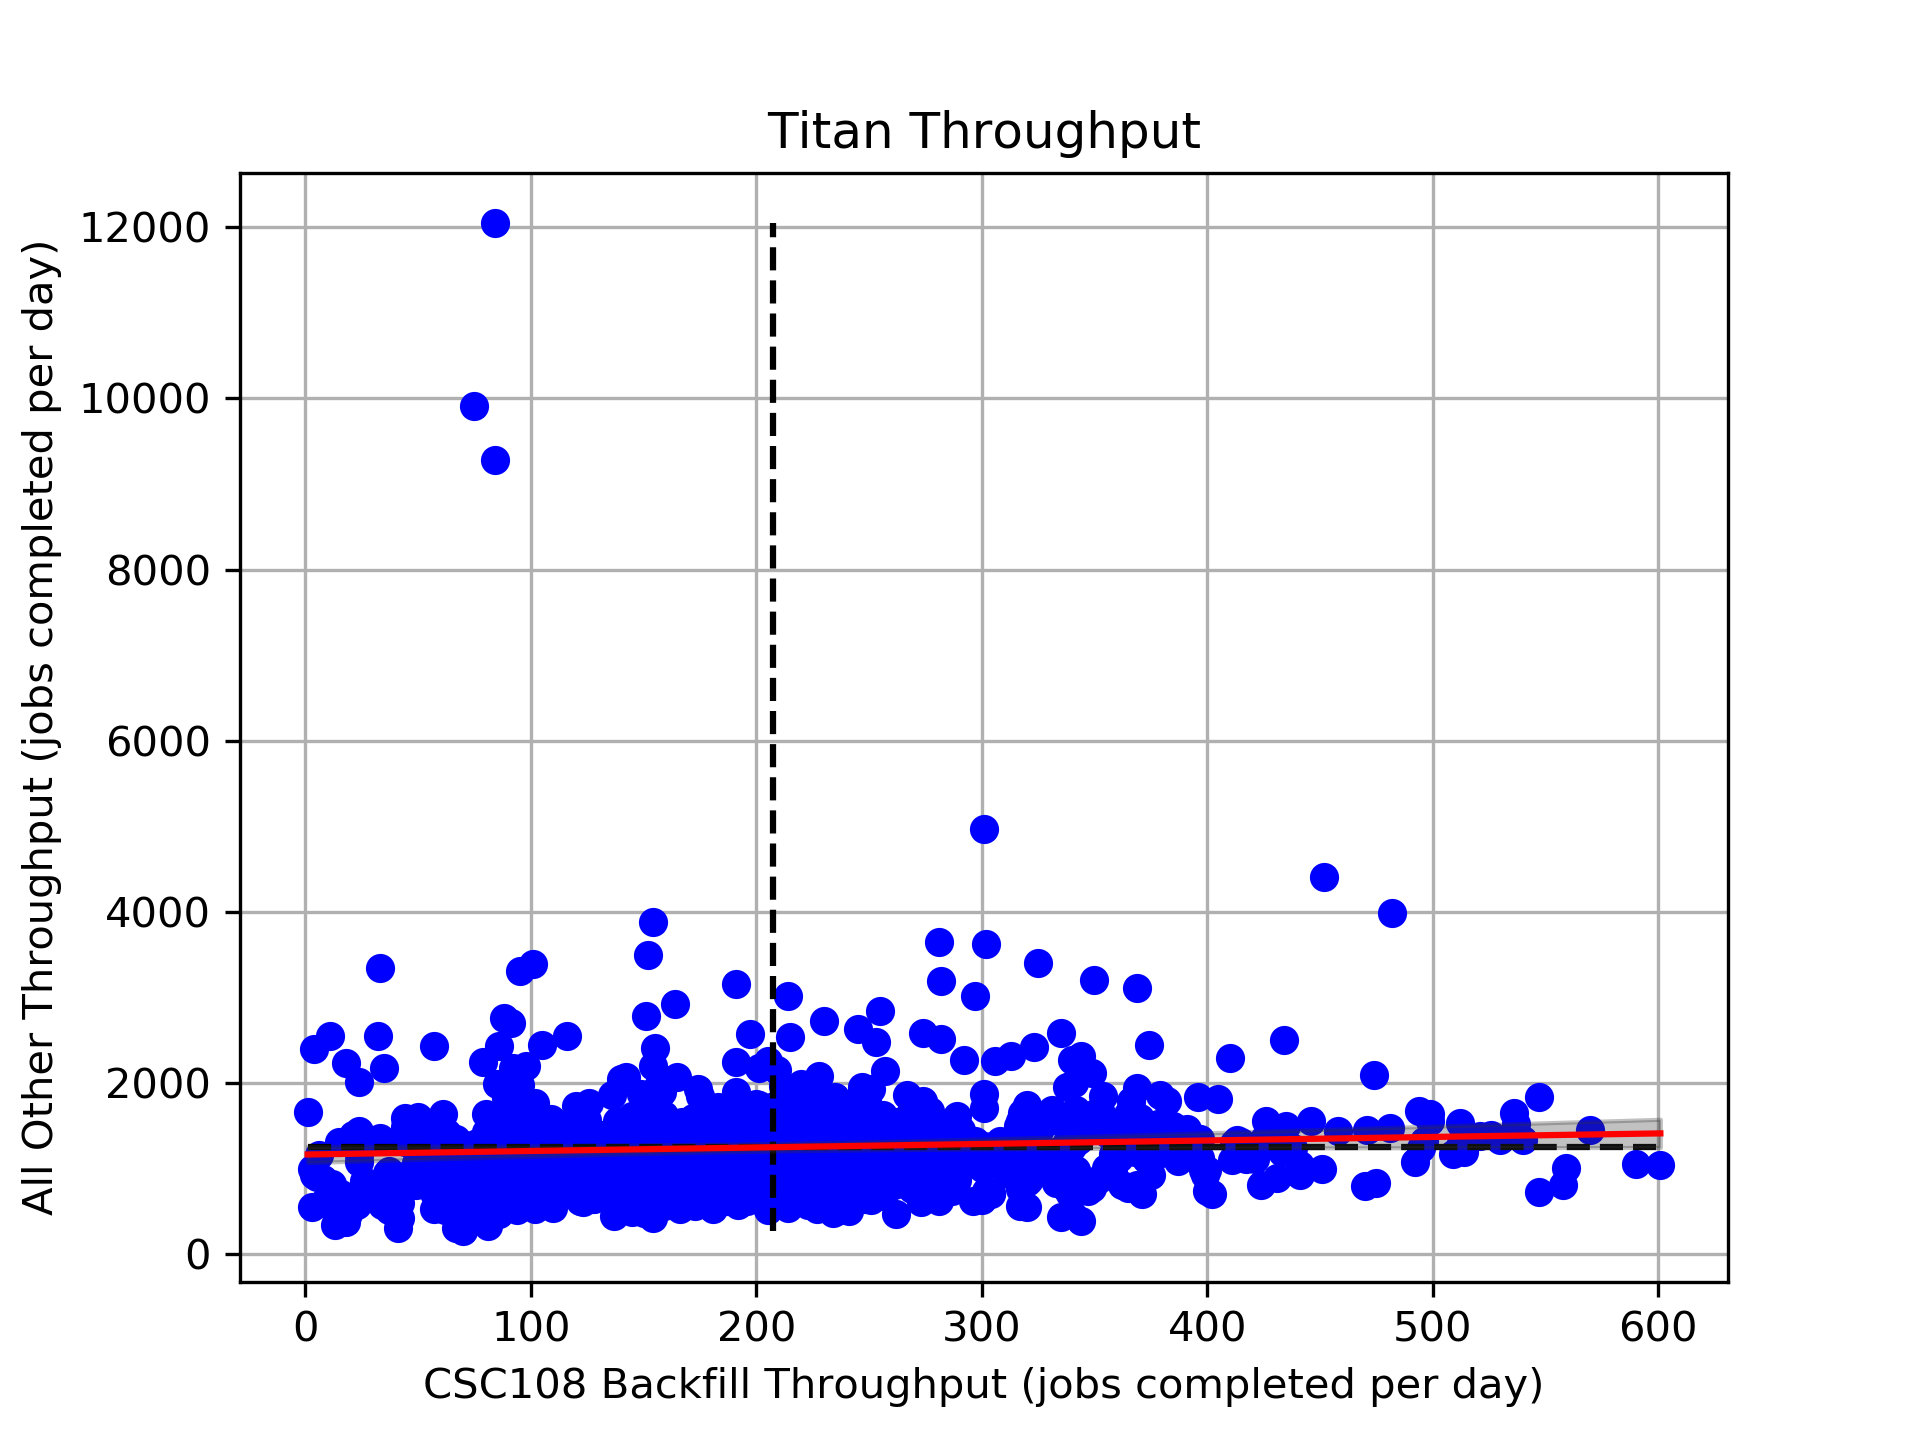
\includegraphics[width=0.75\textwidth]{images/linfit-throughput-all.png}
%% figure caption is below the figure
%\caption{This figure shows the relationship between CSC108 backfill throughput
%and overall throughput by counting jobs completed by day.}
%\label{fig:throughput-all}
%\end{figure*}

%%%%%%%%%%%%%%%%%%%%%%%%%%%%%%%%%%%%%%%%%%%%%%%%%%%%%%%%%%%%%%%%%%%%%%%%%%%%%%%

The PanDA team, known primarily by the project identifier ``CSC108'' at Oak
Ridge, began work on this project in 2013, and our opportunistic consumption of
backfill resources on Titan has increased steadily every year. During this time
period, overall utilization on Titan has increased as well, which is consistent
with our expectations because CSC108 seeks to consume time-sensitive resources
that would otherwise go to waste. The simple bar plot shown in
Figure~\ref{fig:jacks-slide} was created to visualize this progress over time,
and interestingly, it also shows that utilization by other projects has been
decreasing over the same time period. A first reaction when observing this
pattern might be to blame CSC108 for crowding out other projects on Titan, but
careful consideration reveals that there are many other mechanisms which might
be behind these effects. Consequently, we undertook several studies in order to
assess the impact CSC108 is having on Titan and its users, especially with
respect to wait times, throughput, and utilization. This section presents
results from several ongoing studies.

% For two-column wide figures use
\begin{figure*}
% Use the relevant command to insert your figure file.
% For example, with the graphicx package use
  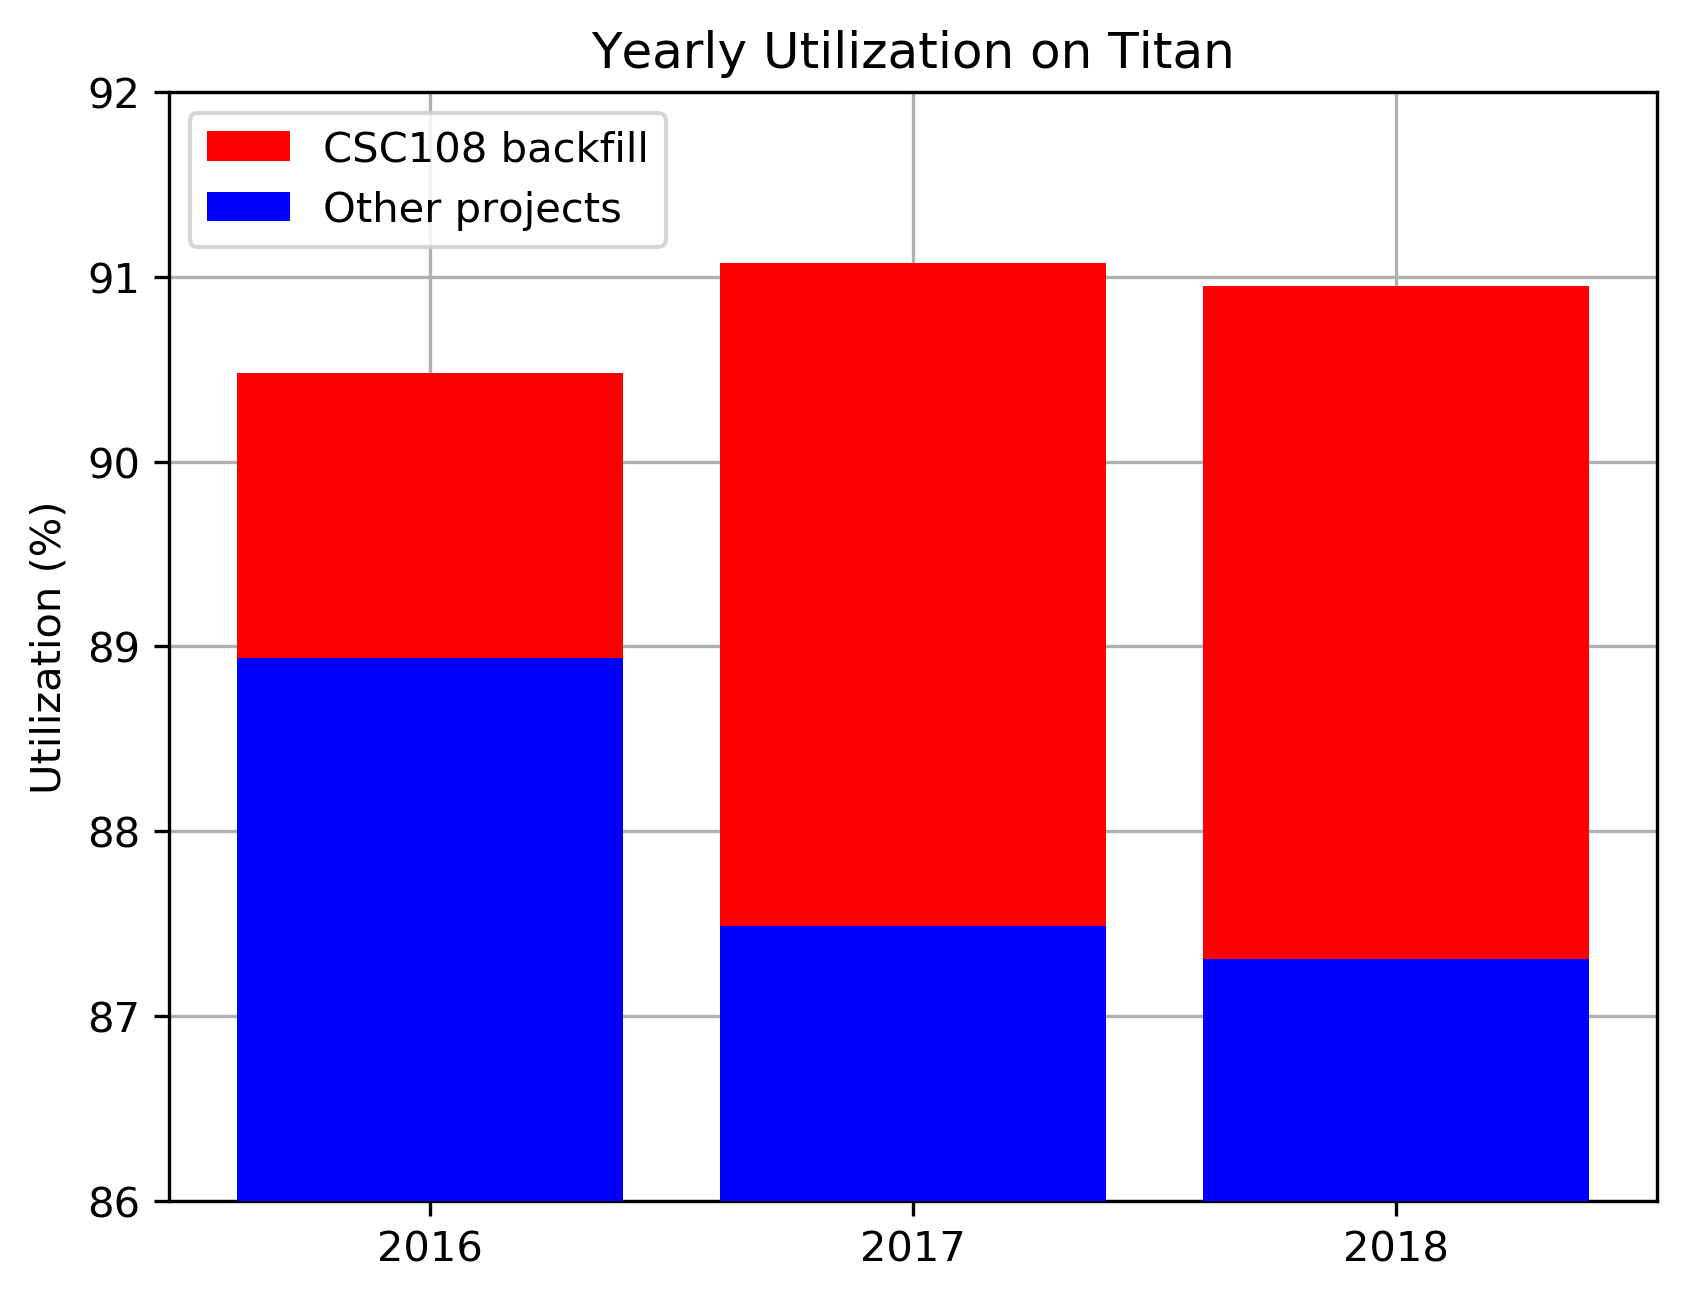
\includegraphics[width=0.75\textwidth]{images/barplot-jacks-slide.png}
% figure caption is below the figure
\caption{This bar plot visualizes the yearly utilization of Titan core hours,
separated into two categories: CSC108's utilization of Titan core hours through
backfill opportunities (shown in red), and all other utilization of core hours
on Titan (shown in blue). The data for 2018 are incomplete; they cover from
January 1, 2018 to October 15, 2018.}
\label{fig:jacks-slide}
\end{figure*}


Before presenting results, however, it is important to summarize the relevant
policies at Oak Ridge for running jobs on Titan. There are three queues on
Titan: batch, debug, and killable. There is no actual backfill queue on Titan;
instead, smaller jobs from each queue are scheduled into spaces that cannot be
used by larger jobs. The batch queue is the default queue for submitted jobs,
and it is the only queue considered in this analysis. Jobs submitted to the
batch queue are grouped into five ``bins'' according to the number of requested
nodes, and each bin has a maximum wall time. Jobs that request fewer nodes have
correspondingly lesser maximum wall times. The definitions and rules for each
bin are shown in Table~\ref{tab:olcfbins}. Nodes are assigned exclusively to
one job at a time. Because Titan is a leadership class machine and priority is
a function of wait time, the batch scheduler awards aging boosts to jobs in
bins 1 and 2 in order to prioritize larger jobs over smaller ones. Once jobs in
the batch queue begin to run, however, they will not be killed when new jobs
arrive, regardless of their priority. Sometimes, jobs small enough to use
currently idle resources on Titan are scheduled to run immediately, and this is
what we refer to as ``backfill opportunity''. CSC108 takes advantage of the
``showbf'' command in order to query the Moab scheduler directly for currently
available backfill opportunity and then tailors its own submissions to Titan
accordingly. CSC108 has a special policy applied to guarantee that its jobs run
with lesser priority than all others on Titan, to ensure that its jobs consume
only backfill resources. Finally, ``Titan core hours'' are the billable units
used at OLCF; they convert at a rate of 30 Titan core hours per 1 node hour.

% For tables use
\begin{table}
% table caption is above the table
\caption{OLCF policies sort jobs into numbered bins based on the requested
number of nodes, and each bin has its own set of constraints.}
\label{tab:olcfbins}       % Give a unique label
% For LaTeX tables use
\begin{tabular}{crrr}
\hline\noalign{\smallskip}
Bin & Requested Nodes   & Maximum Wall Time &   Aging Boost \\
\noalign{\smallskip}\hline\noalign{\smallskip}
1   &   11,250 - 18,688 &   24 hours        &   15 days     \\
2   &    3,750 - 11,249 &   24 hours        &    5 days     \\
3   &       313 - 3,749 &   12 hours        &         0     \\
4   &         126 - 312 &    6 hours        &         0     \\
5   &           1 - 125 &    2 hours        &         0     \\
\noalign{\smallskip}\hline
\end{tabular}
\end{table}


% For two-column wide figures use
\begin{figure*}
% Use the relevant command to insert your figure file.
% For example, with the graphicx package use
  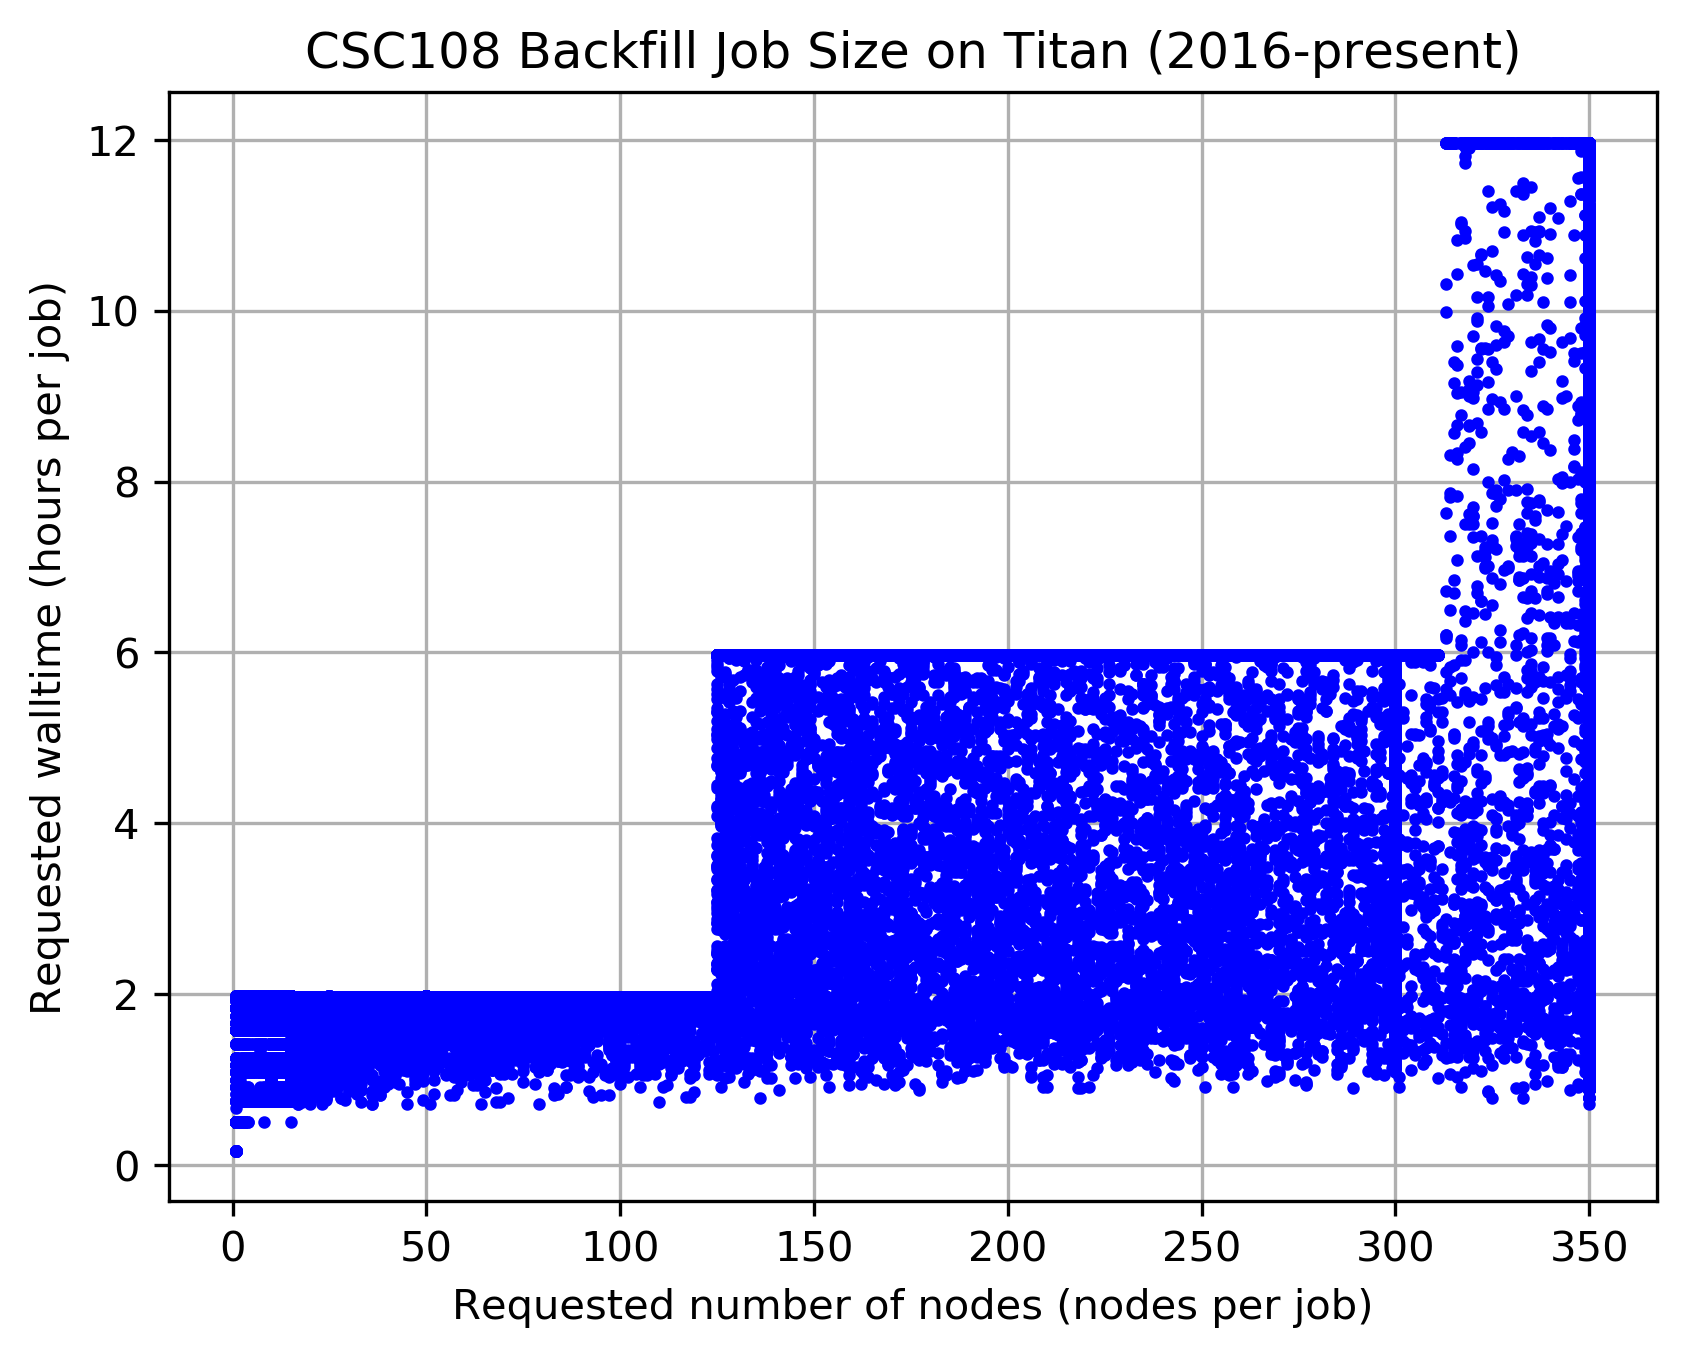
\includegraphics[width=0.75\textwidth]{images/time-vs-nodes-backfill.png}
% figure caption is below the figure
\caption{This figure shows that the PanDA deployment on Titan runs CSC108 jobs
that vary in size by time and by space. The stair steps occur due to the
constraints from Titan policy by bin. The jobs in the bottom left ``column''
run in bin 5, the jobs in the middle are running in bin 4, and the jobs on the
right are bin 3. Note that the rightmost boundary of the plot, at 350 nodes,
represents a self-imposed constraint.}
\label{fig:time-vs-nodes}
\end{figure*}

The studies have collected datasets in several different ways. Initially, we
began by sampling live data from Moab by polling with Python scripts launched
by cron jobs on a data transfer node. These scripts recorded XML output from
the ``showbf'' and ``showq'' commands into files, and more cron jobs launched
other Python scripts to import these files' sample data into SQLite. These
tables contain data about the exact state of the queues at given times,
including active jobs, blocked jobs, eligible jobs, recently completed jobs,
and system information such as active nodes and available backfill
opportunities. We then supplemented these live samples with daily availability
data and historical job traces obtained from ORNL. The daily availability data
span from January 1, 2016 to October 18, 2018 and contain only the total Titan
core hours that were available each day. The historical job trace data span
from January 1, 2016 to October 15, 2018 and contain only job submission time,
start time, completion time, requested nodes, and requested wall time, for all
jobs not due to the PanDA team. Besides CSC108, the PanDA team has two other
PanDA projects on Titan, which are HEP110 and HEP113, both of which use PanDA
to submit jobs with the increased priority of their ALCC allocations. Thus,
traces for the PanDA jobs contain additional fields for account name, job name,
and user name to distinguish the backfill jobs from the ``direct mode'' jobs.
Finally, we analyzed the SQLite data in Python using the well-known Matplotlib,
NumPy, and SciPy libraries via Anaconda.

%%%%%%%%%%%%%%%%%%%%%%%%%%%%%%%%%%%%%%%%%%%%%%%%%%%%%%%%%%%%%%%%%%%%%%%%%%%%%%%%
\subsection{Wait Times}
\label{subsec:waittimes}

First, we discuss the impact of CSC108's jobs on the wait times experienced by
other projects' jobs on Titan.

%%%%%%%%%%%%%%%%%%%%%%%%%%%%%%%%%%%%%%%%%%%%%%%%%%%%%%%%%%%%%%%%%%%%%%%%%%%%%%%%
\subsubsection{Blocking Model}
\label{subsubsec:blockingmodel}

We began by developing a simple model to estimate how often that a CSC108 job
was using resources on Titan that would have been used by another project's job
if they had been available. To this end, we defined an abstract event called a
``block'' and then detected occurrences of the event within our data.

Let $C_i$ be the abstract resources in use by CSC108 at the $i^{\text{th}}$
sample point in time, and let $U_i$ be the unused (idle) resources remaining on
Titan. We then define a boolean $B_i$ representing a ``block'' to be 1 if there
exists at least one job at the $i^{\text{th}}$ sample point which requests
$(C_i + U_i)$ resources or less when $C_i$ is non-zero; we define $B_i$ to be
zero otherwise. Summing $B_i$ over all $i$ gives a count of sample points at
which a block occurred, and dividing that count by the number of total sample
points yields a quantity we call a ``blocking fraction''. The blocking fraction
is a rational number between 0 and 1, with lesser numbers corresponding to
lesser impacts by CSC108.

To apply this abstract model to a real data set, we have initially defined the
resources in a purely ``spatial'' manner by considering only jobs' requested
numbers of nodes. Further work will explore ``spatiotemporal'' blocking by also
considering jobs' requested wall times.


% For two-column wide figures use
\begin{figure*}
% Use the relevant command to insert your figure file.
% For example, with the graphicx package use
  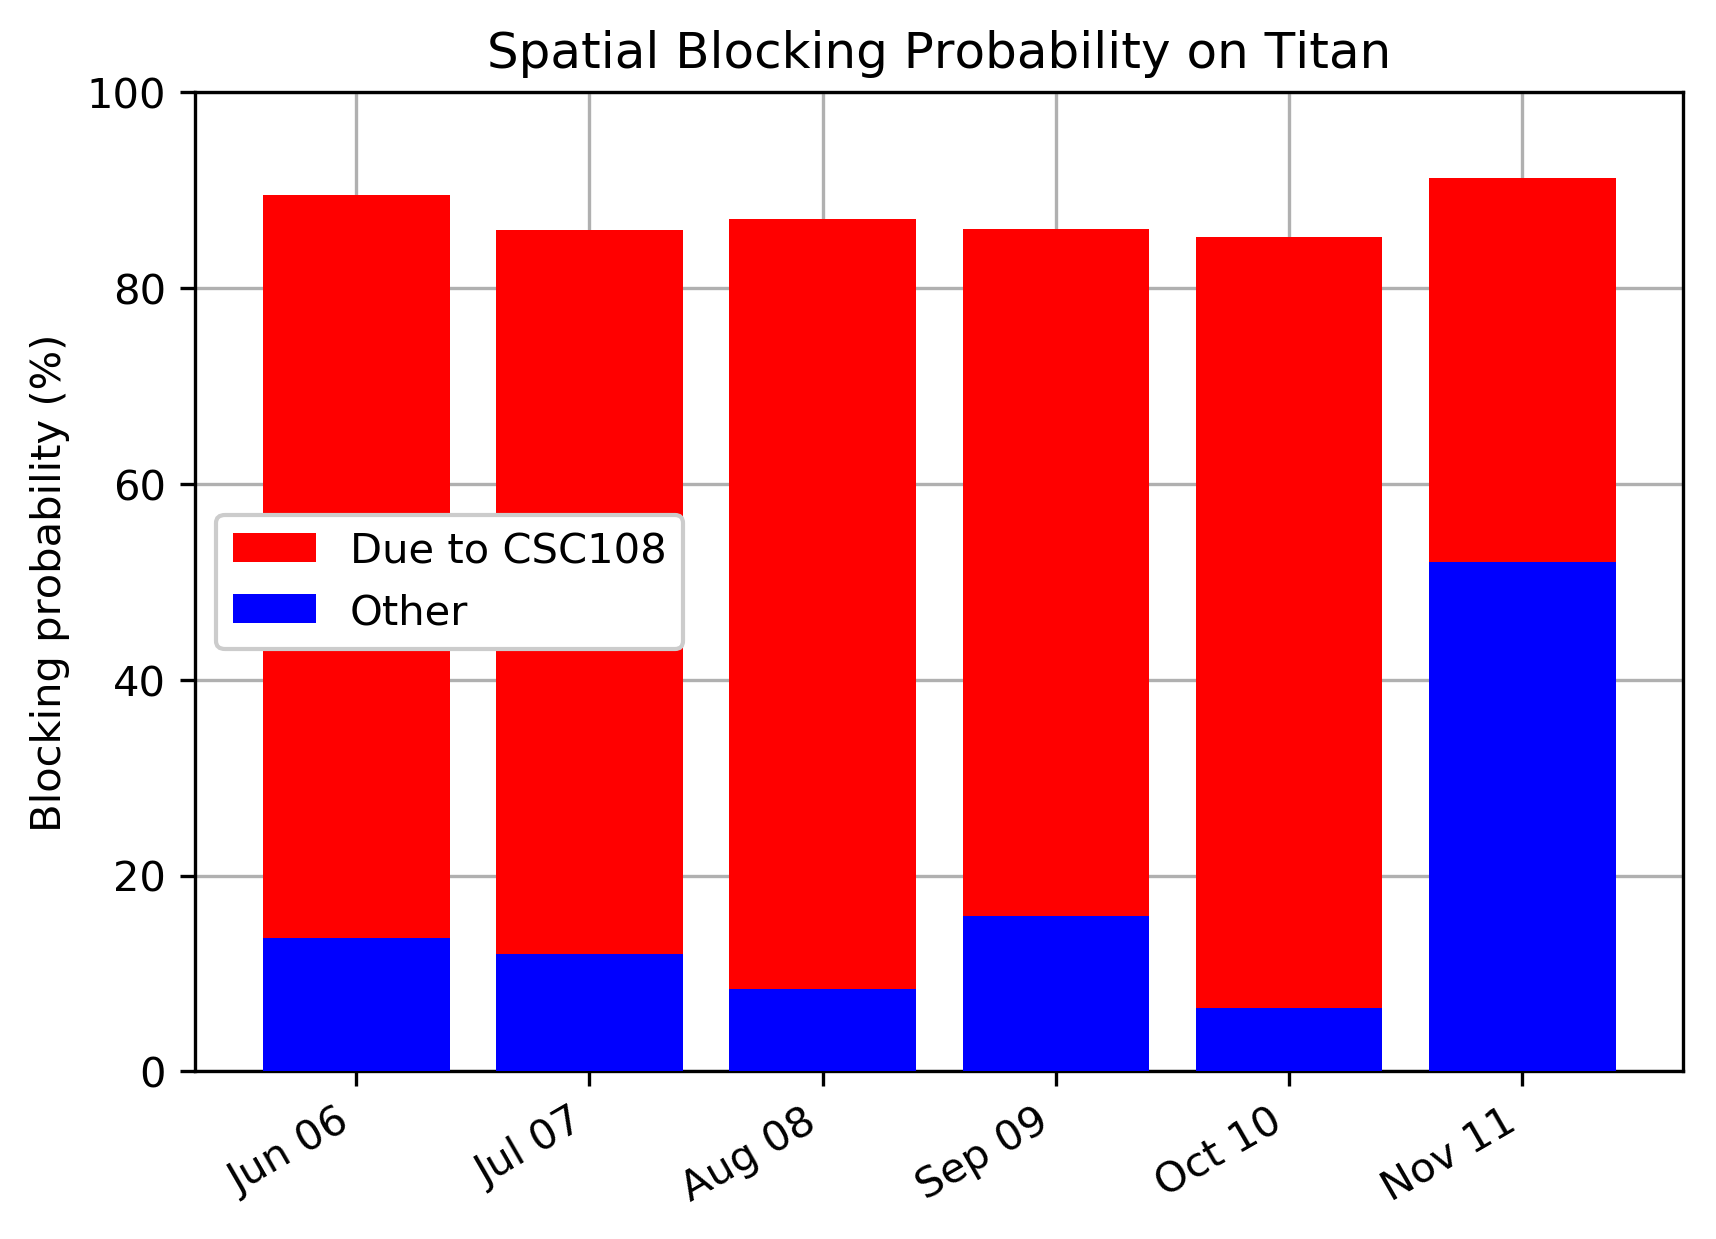
\includegraphics[width=0.75\textwidth]{images/barplot-spatial-blocking-by-month.png}
% figure caption is below the figure
\caption{This figure shows the spatial blocking probabilities by month for
samples where CSC108 was actively utilizing backfill opportunity. An eligible
job in the batch queue is said to be blocked spatially when the job's number of
requested nodes is too large to fit within the nodes available through backfill
opportunity, so that the job must wait to run. The total height of the bars
indicates the spatial blocking probability for the month, which is the
percentage of samples in which at least one eligible job was spatially blocked.
The red region indicates the percentage of samples in which at least one
eligible job would no longer be spatially blocked if CSC108 freed its
resources.}
\label{fig:spatial-blocking-by-month}
\end{figure*}


% For two-column wide figures use
\begin{figure*}
% Use the relevant command to insert your figure file.
% For example, with the graphicx package use
  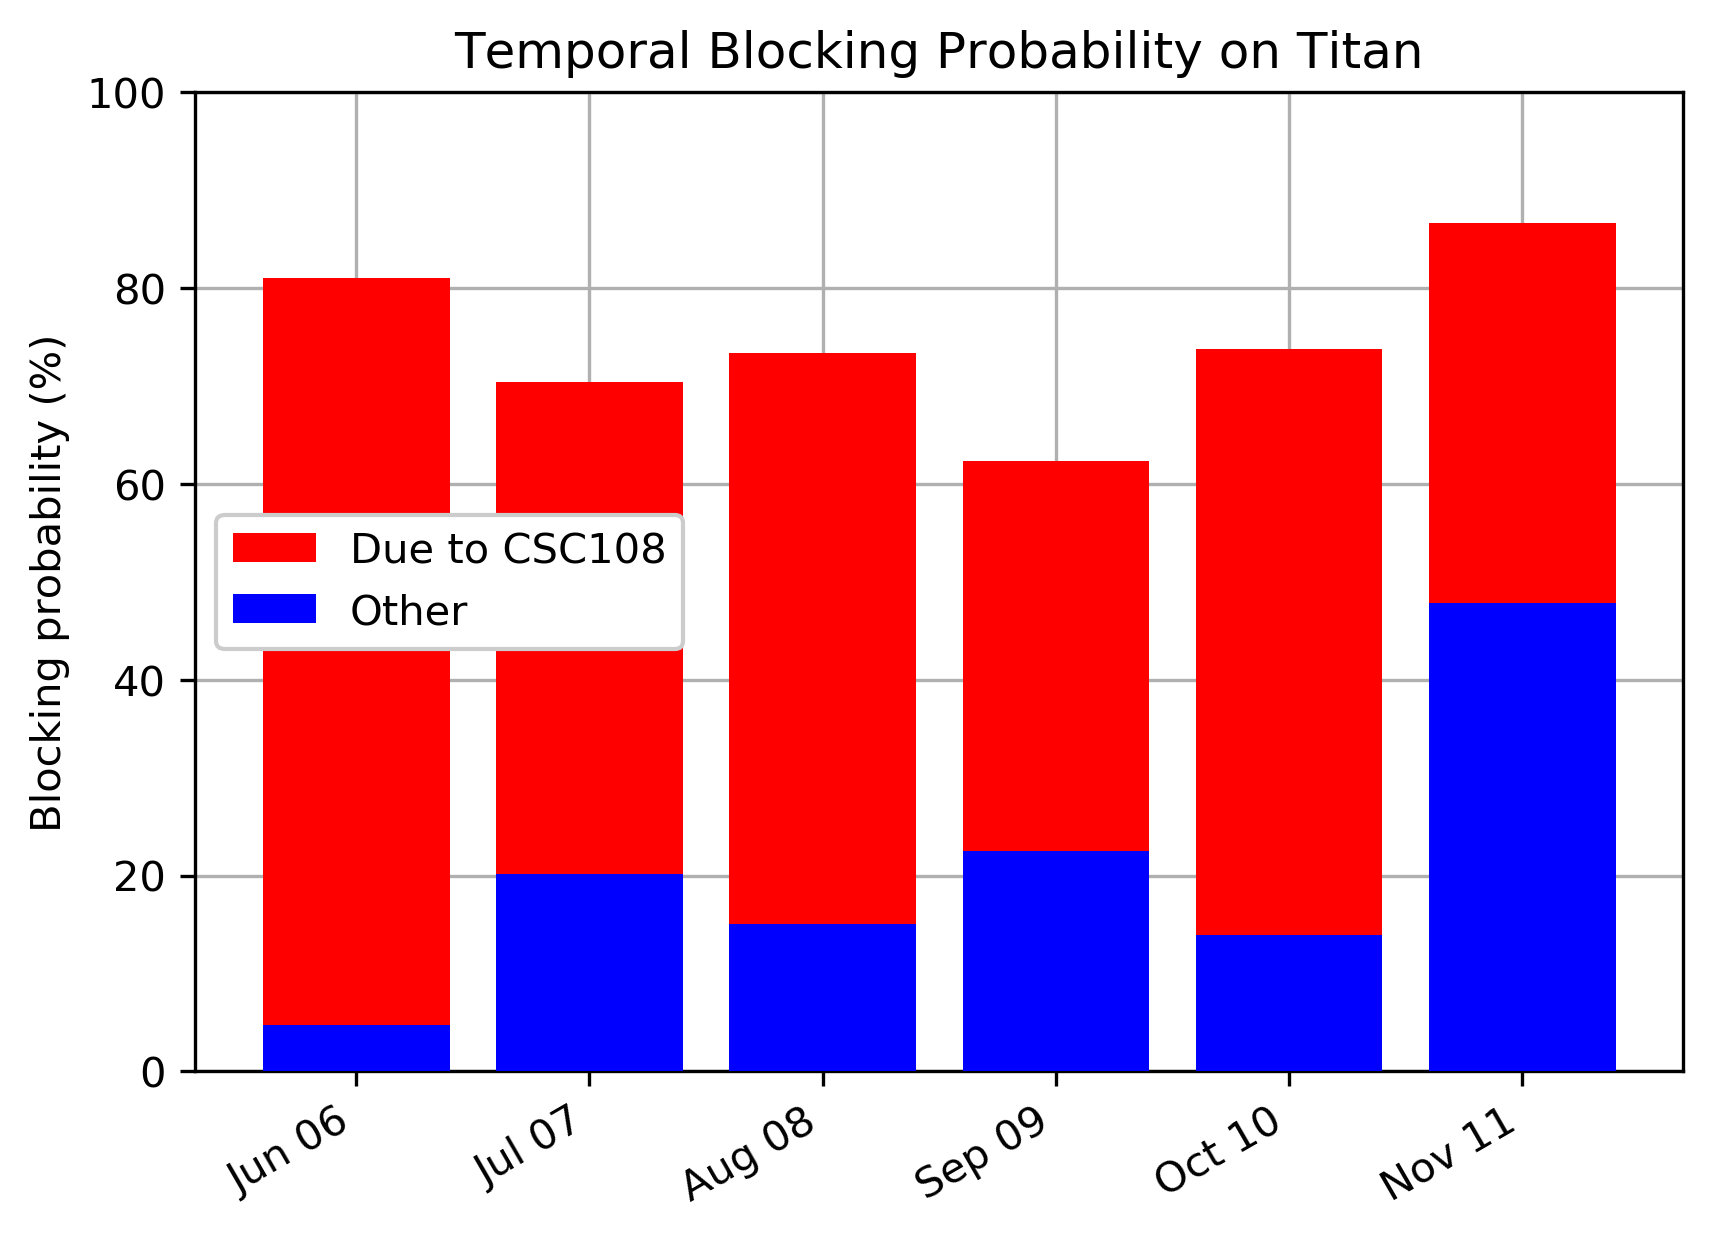
\includegraphics[width=0.75\textwidth]{images/barplot-temporal-blocking-by-month.png}
% figure caption is below the figure
\caption{This figure shows the temporal blocking probabilities by month for
samples where CSC108 was actively utilizing backfill opportunity.An eligible
job in the batch queue is said to be blocked temporally when the job's
requested wall time is too long to fit within the duration available through
backfill opportunity, so that the job must wait to run. The total height of the
bars indicates the temporal blocking probability for the month, which is the
percentage of samples in which at least one eligible job was temporally
blocked. The red region indicates the percentage of samples in which at least
one eligible job would no longer be temporally blocked if CSC108 freed its
resources.}
\label{fig:temporal-blocking-by-month}
\end{figure*}


%%%%%%%%%%%%%%%%%%%%%%%%%%%%%%%%%%%%%%%%%%%%%%%%%%%%%%%%%%%%%%%%%%%%%%%%%%%%%%%%
\subsubsection{Dormant period}
\label{subsubsec:dormantperiod}

An interesting opportunity arose during July 2018 following the end of a large
simulation campaign by ATLAS, because CSC108 submitted zero backfill jobs for
14 consecutive days. For convenience, we have called this the ``dormant
period''. This unusually long dormant period allows comparison of the system
when CSC108 is running versus the system when CSC108 is completely absent.

Prior to the dormant period, CSC108 had consumed an average of 7.5 million
Titan core hours every two weeks during the first six months of 2018.



\textbf{Keep going.}


%%%%%%%%%%%%%%%%%%%%%%%%%%%%%%%%%%%%%%%%%%%%%%%%%%%%%%%%%%%%%%%%%%%%%%%%%%%%%%%%
\subsection{Throughput}
\label{subsec:throughput}


Next, we discuss the impact of CSC108's jobs on throughput on Titan. We modeled
the relationships between overall throughput on Titan, in units of jobs
completed per day, with CSC108's overall throughput and also with its
throughputs when separated by OLCF bin number. The resulting models are shown
in Figures~\ref{fig:throughput-all}, \ref{fig:throughput-bin3},
\ref{fig:throughput-bin4}, and \ref{fig:throughput-bin5}.

% For tables use
\begin{table}
% table caption is above the table
\caption{(placeholder caption)}
\label{tab:throughput-params}       % Give a unique label
% For LaTeX tables use
\begin{tabular}{ccrr}
\hline\noalign{\smallskip}
Figure  &   Bin & Slope   & Intercept   \\
\noalign{\smallskip}\hline\noalign{\smallskip}
\ref{fig:throughput-all}    &   All &   0.6797  &   1184.1510   \\
\ref{fig:throughput-bin3}   &   3   &  -0.7029  &   1742.0276   \\
\ref{fig:throughput-bin4}   &   4   &   5.7949  &   1427.9643   \\
\ref{fig:throughput-bin5}   &   5   &   0.6200  &   1249.8151   \\
\noalign{\smallskip}\hline
\end{tabular}
\end{table}

All four of the models share common parameters, which can be viewed in
Table~\ref{tab:throughput-params}. Each model has a small magnitude slope in
relation to the magnitude of its Y intercept, which indicates that the impact
of increased throughput by CSC108 is small in each model. Each model appears to
be a relatively flat line positioned at approximately 1400 jobs completed per
day on Titan.

These results are consistent with our intuition about the behavior of Titan
when the Moab scheduler begins ``draining'' in order to accommodate leadership
class jobs. During the draining process, the nodes of completed jobs are not
immediately reassigned, because the Moab scheduler reserves them in order to
run a leadership class job in the future. Moab will only schedule jobs to run
on those now-idle nodes if they will complete before the leadership class job's
reservation begins. Thus, just before large jobs, which decrease overall
throughput, run on Titan, more backfill opportunities arise for small jobs,
which increase throughput; this effect helps Titan maintain its overall level
of throughput. Because PanDA submits jobs of different sizes according to
available backfill opportunity, as shown in Figure~\ref{fig:time-vs-nodes},
CSC108's throughput minimally impacts Titan's overall throughput.

% For two-column wide figures use
\begin{figure*}
% Use the relevant command to insert your figure file.
% For example, with the graphicx package use
  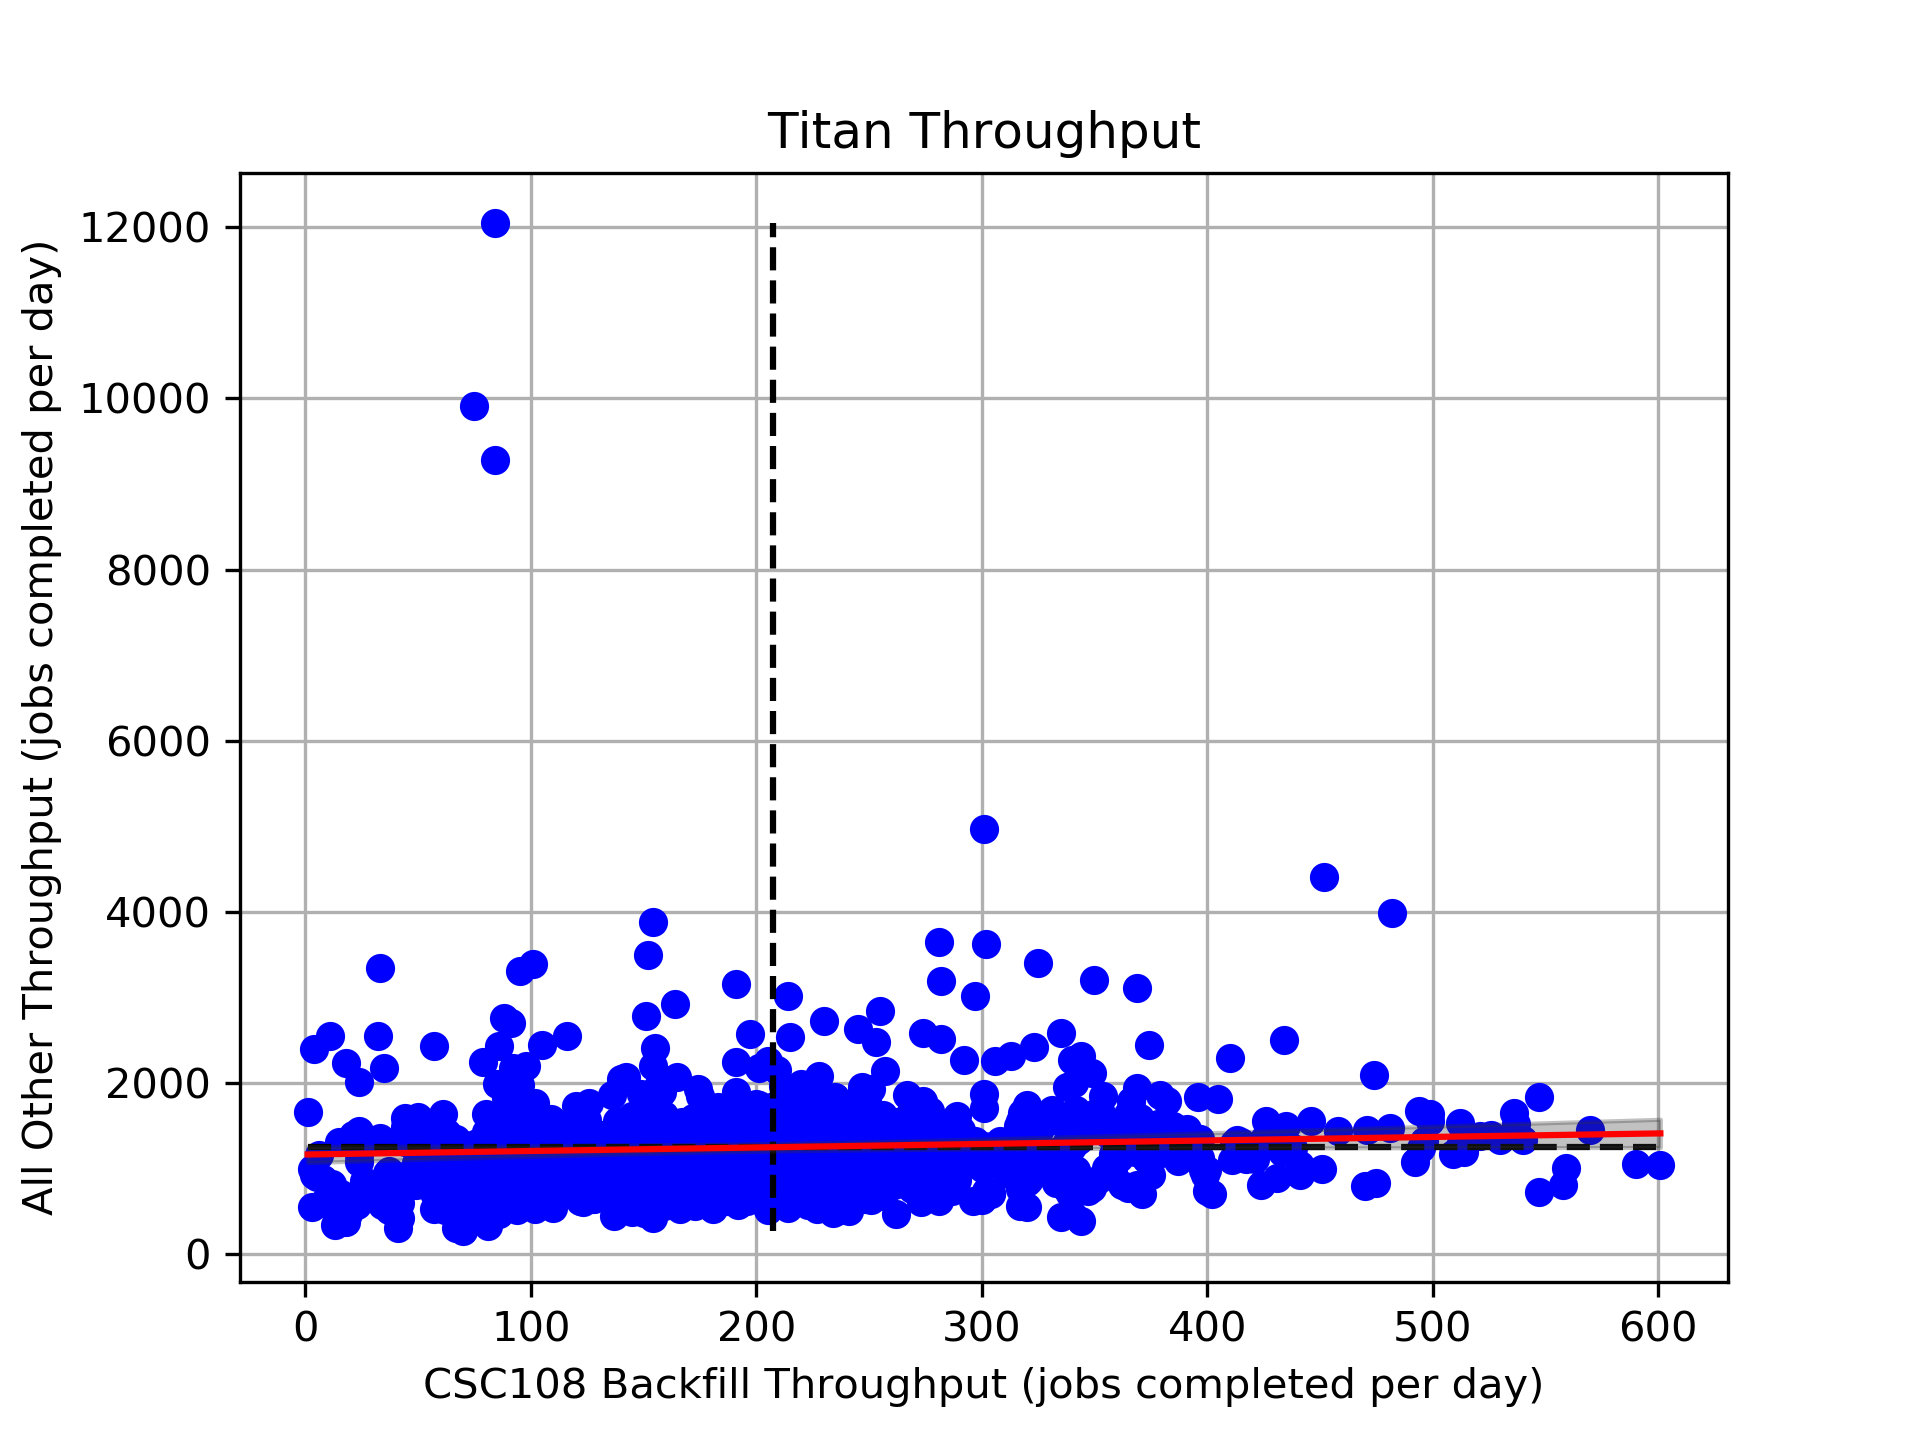
\includegraphics[width=0.75\textwidth]{images/linfit-throughput-all.png}
% figure caption is below the figure
\caption{Parameters for the model are shown in
    Table~\ref{tab:throughput-params}.}
\label{fig:throughput-all}
\end{figure*}

% For two-column wide figures use
\begin{figure*}
% Use the relevant command to insert your figure file.
% For example, with the graphicx package use
  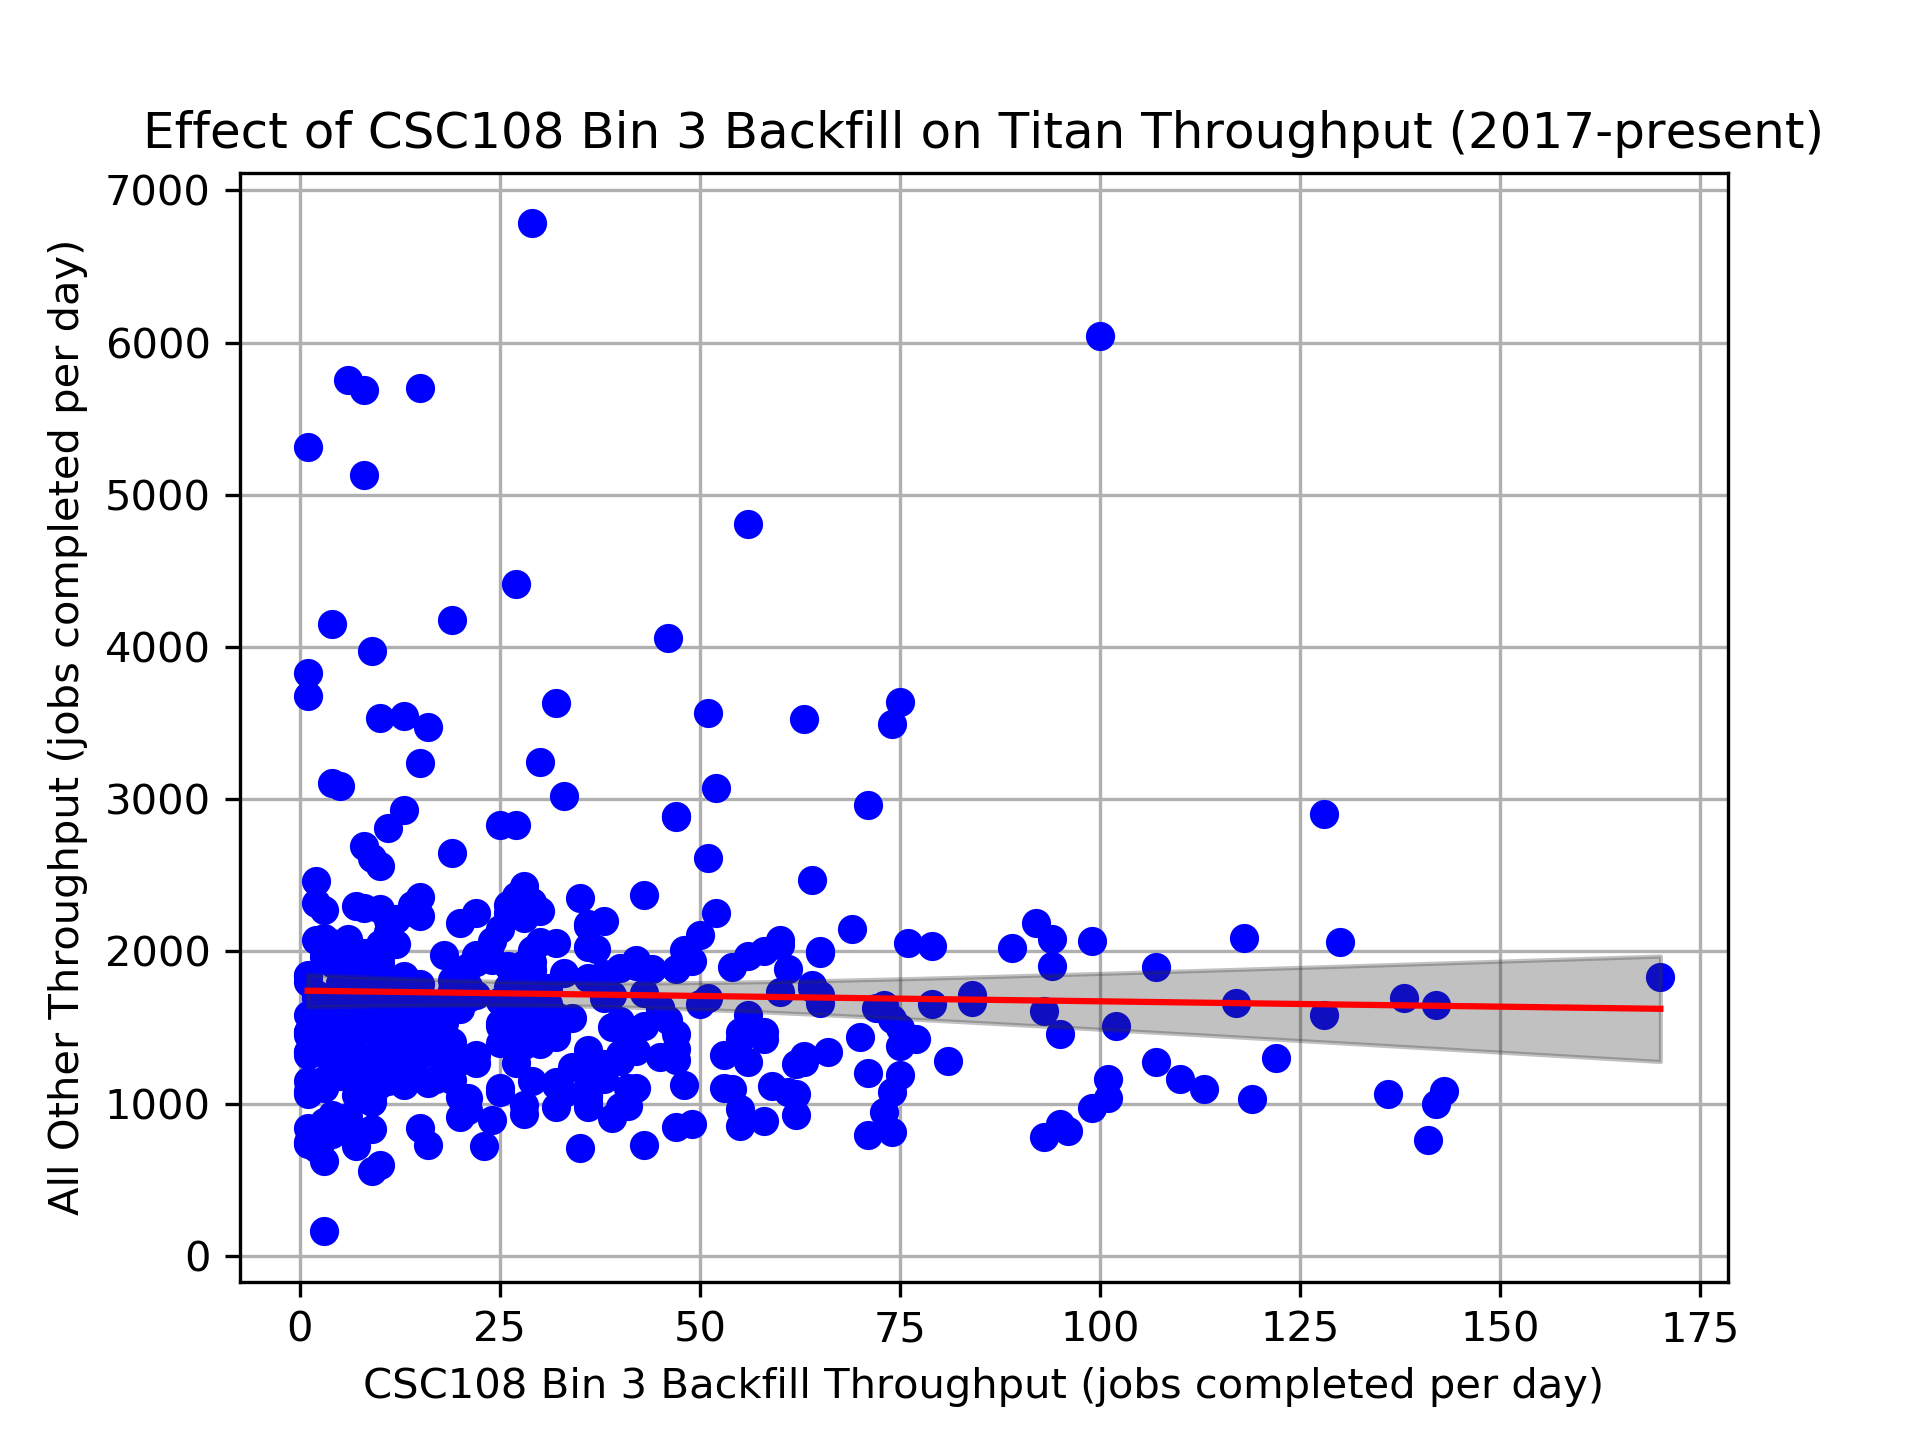
\includegraphics[width=0.75\textwidth]{images/linfit-throughput-bin3.png}
% figure caption is below the figure
\caption{Parameters for the model are shown in
    Table~\ref{tab:throughput-params}.}
\label{fig:throughput-bin3}
\end{figure*}

% For two-column wide figures use
\begin{figure*}
% Use the relevant command to insert your figure file.
% For example, with the graphicx package use
  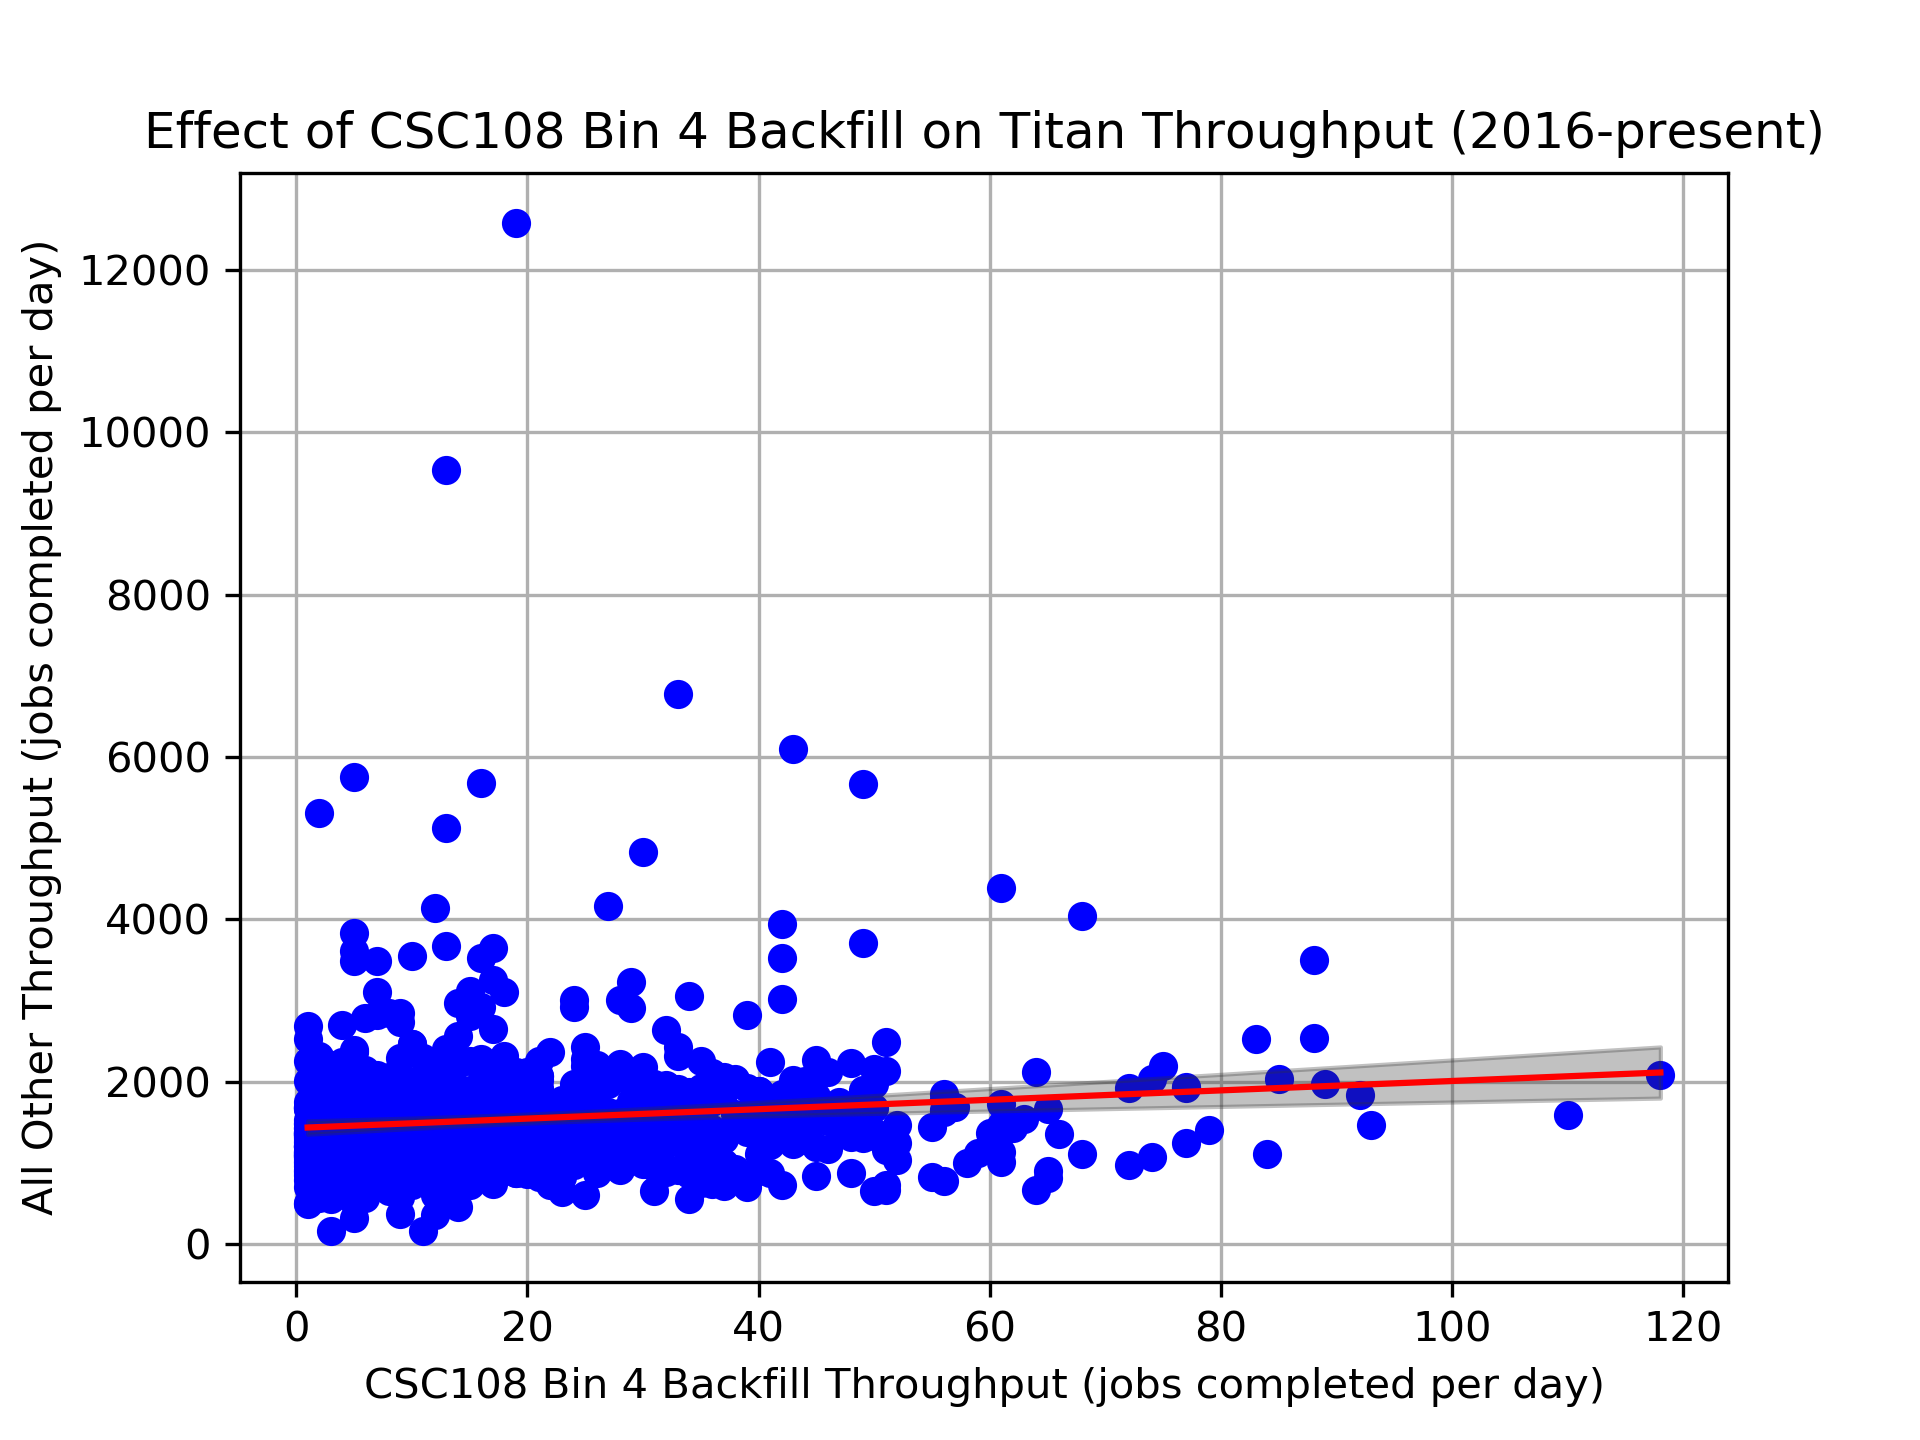
\includegraphics[width=0.75\textwidth]{images/linfit-throughput-bin4.png}
% figure caption is below the figure
\caption{Parameters for the model are shown in
    Table~\ref{tab:throughput-params}.}
\label{fig:throughput-bin4}
\end{figure*}

% For two-column wide figures use
\begin{figure*}
% Use the relevant command to insert your figure file.
% For example, with the graphicx package use
  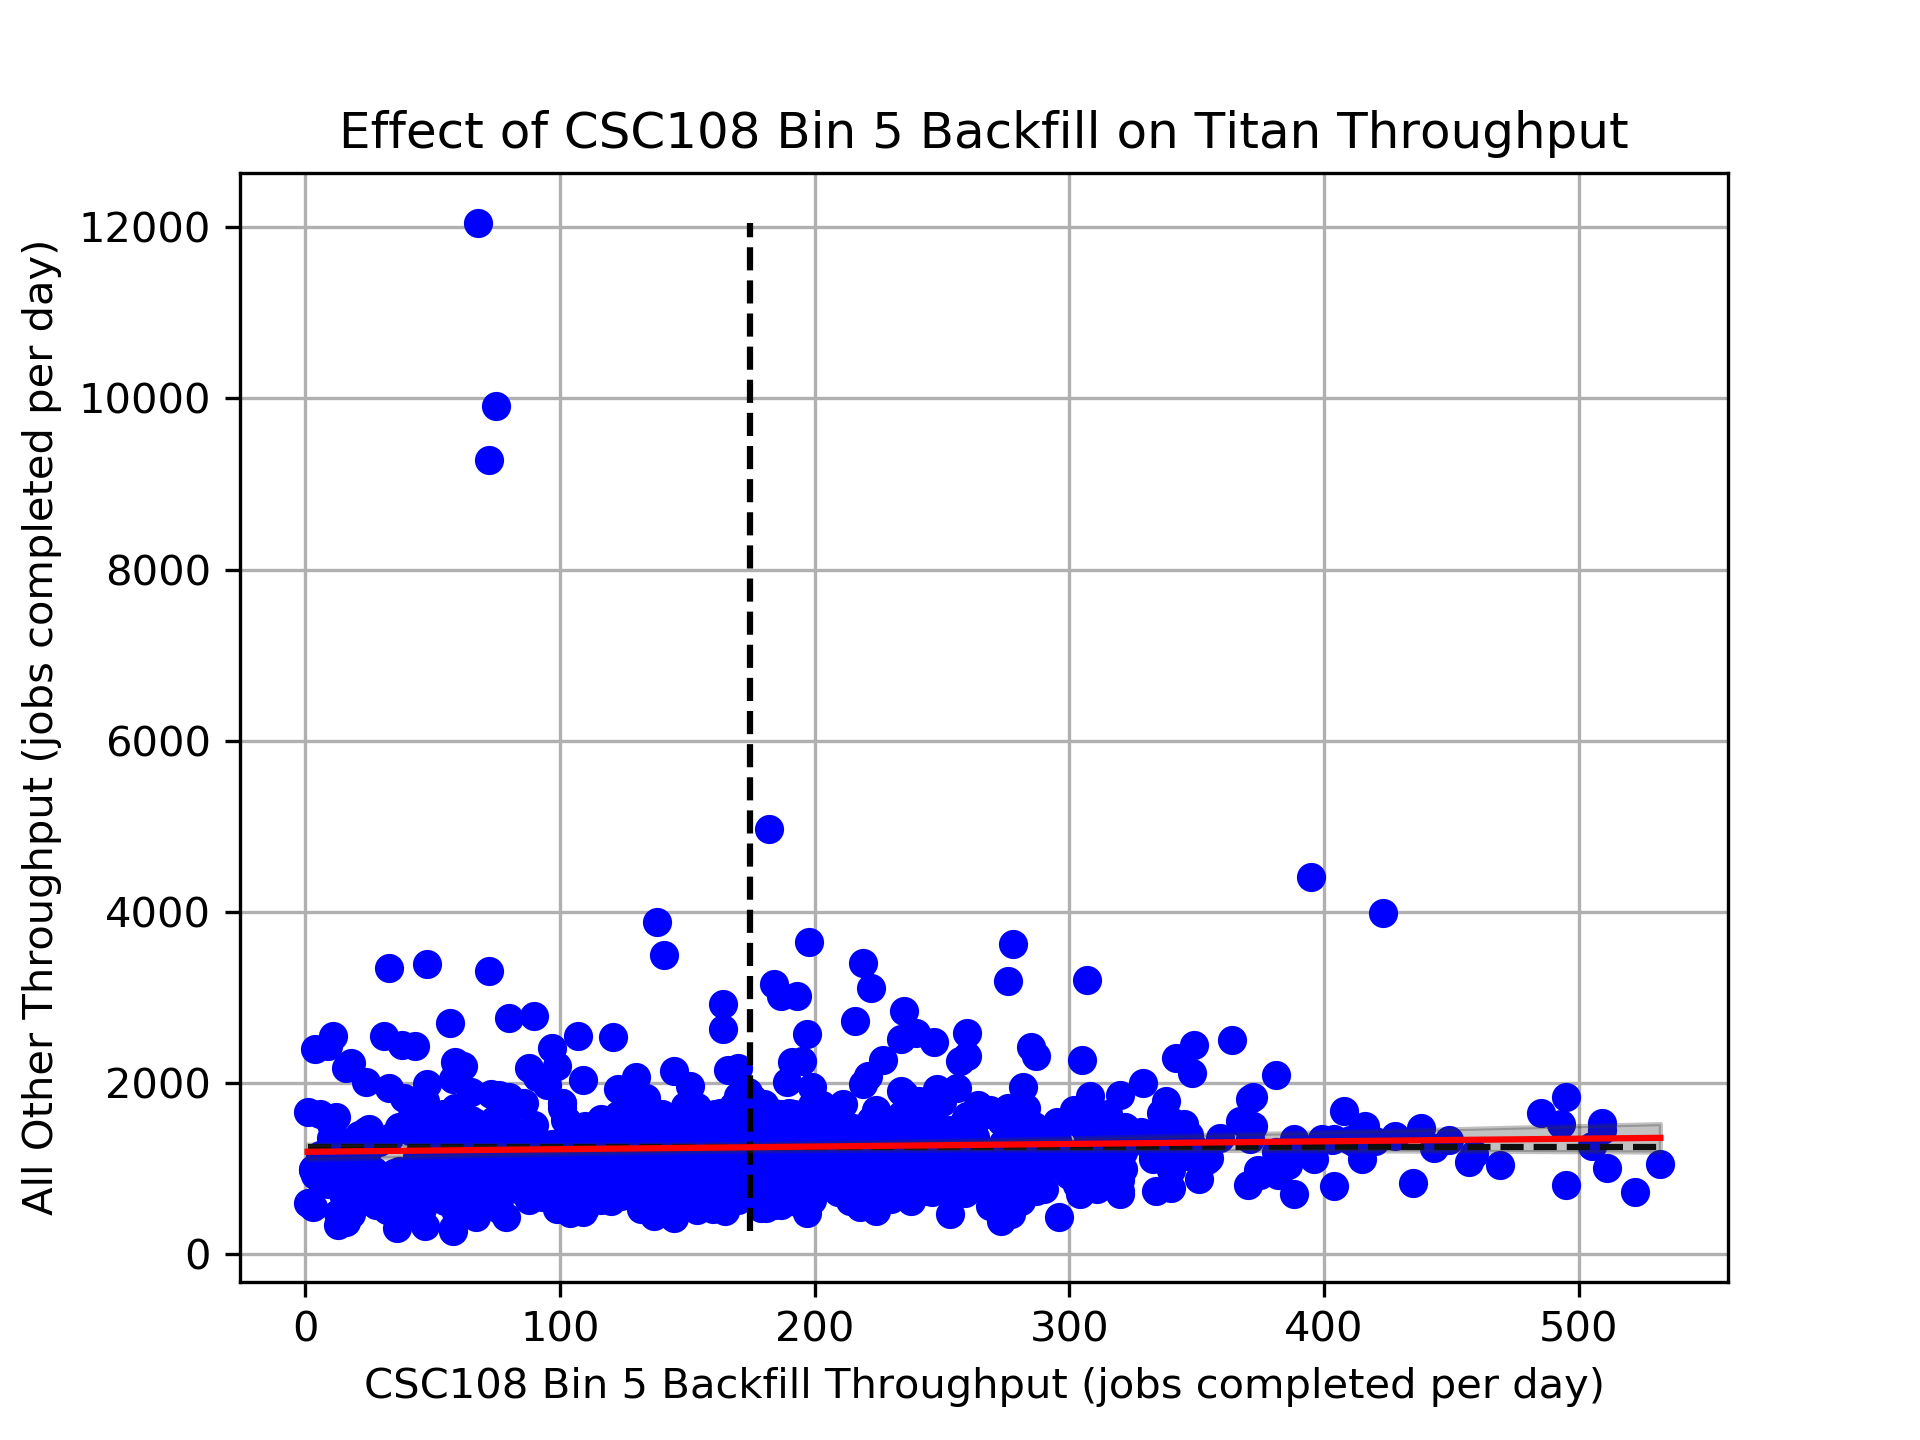
\includegraphics[width=0.75\textwidth]{images/linfit-throughput-bin5.png}
% figure caption is below the figure
\caption{Parameters for the model are shown in
    Table~\ref{tab:throughput-params}.}
\label{fig:throughput-bin5}
\end{figure*}


%%%%%%%%%%%%%%%%%%%%%%%%%%%%%%%%%%%%%%%%%%%%%%%%%%%%%%%%%%%%%%%%%%%%%%%%%%%%%%%%
\subsection{Utilization}
\label{subsec:utilization}

Finally, we are investigating the effects of CSC108's utilization of backfill
opportunity on the overall utilization of Titan by all projects. To do this, we
constructed using linear models again, in a manner very similar to that of
Section~\ref{subsec:throughput}. We modeled the relationships between overall
utilization on Titan, as the percentage of available core hours consumed per
day, with CSC108's utilization and also with its utilizations when separated by
OLCF bin number. The resulting models are shown in
Figures~\ref{fig:utilization-all}, \ref{fig:utilization-bin3},
\ref{fig:utilization-bin4}, and \ref{fig:utilization-bin5}. The parameters of
the models shown in the figures are shown in
Table~\ref{tab:utilization-params}.

% For tables use
\begin{table}
% table caption is above the table
\caption{(placeholder caption)}
\label{tab:utilization-params}       % Give a unique label
% For LaTeX tables use
\begin{tabular}{ccrr}
\hline\noalign{\smallskip}
Figure  &   Bin & Slope   & Intercept   \\
\noalign{\smallskip}\hline\noalign{\smallskip}
\ref{fig:utilization-all}    &   All &  -0.5079 &   93.2965 \\
\ref{fig:utilization-bin3}   &   3   &  -0.8270 &   92.6575 \\
\ref{fig:utilization-bin4}   &   4   &  -1.1121 &   92.8737 \\
\ref{fig:utilization-bin5}   &   5   &  3.9084  &   88.1362 \\
\noalign{\smallskip}\hline
\end{tabular}
\end{table}

Unlike the case for the throughput models in Section~\ref{subsec:throughput},
the parameters shown in Table~\ref{tab:utilization-params} show that one of the
models is not like the others. Although three of the models have very similar
negative slopes and Y intercepts, the model for CSC108's utilization of bin 5
has a positive slope and a Y intercept that is much more interesting.

Titan's overall utilization from January 1, 2017 to October 1, 2018 was
91.9\%, as shown in Figure~\ref{fig:jacks-slide}, and during this same time
period, CSC108's utilization of Titan was about 3.5\%. Given the original
assumption by the project that CSC108 uses only time-sensitive resources which
would have otherwise gone to waste, the natural conclusion is that CSC108's
utilization represents a pure increase in overall utilization, and therefore
that Titan's utilization without CSC108 would have been 88.4\%. By way of
comparison, the bin 5 model predicts this value to be 88.1\%, which is
surprisingly close for such a simple model. The bin 5 model also intercepts
100\% Titan utilization when CSC108 bin 5 utilization is almost exactly 3\%,
which is a feasible number that is similar to the observed overall utilization
by CSC108 of 3.5\%.

The similarity of the parameters of the bin 5 model to the observed values in
the data suggests that Titan's overall utilization is more sensitive to
CSC108's utilization of bin 5 jobs, which are the smallest jobs that run on
Titan. The slope of the bin 5 model is harder to interpret. A slope of 3.9084
in the model suggests that a 1\% increase in utilization by CSC108 in bin 5
results in a roughly 4\% increase in overall utilization. Obviously, a 1\%
increase by CSC108 can only directly result in a 1\% overall increase, but
another reason may be behind this. For example, because CSC108 submits jobs to
bins 3, 4, and 5 consistently, an increase in utilization in bin 5 also
corresponds to a shift away from bins 3 and 4, where the individual models
indicate that increased utilization negatively impacts overall utilization on
Titan. Because we do not yet know the exact mechanism at work here, we are
continuing to pursue this study in order to optimize our job sizing algorithm.


% For two-column wide figures use
\begin{figure*}
% Use the relevant command to insert your figure file.
% For example, with the graphicx package use
  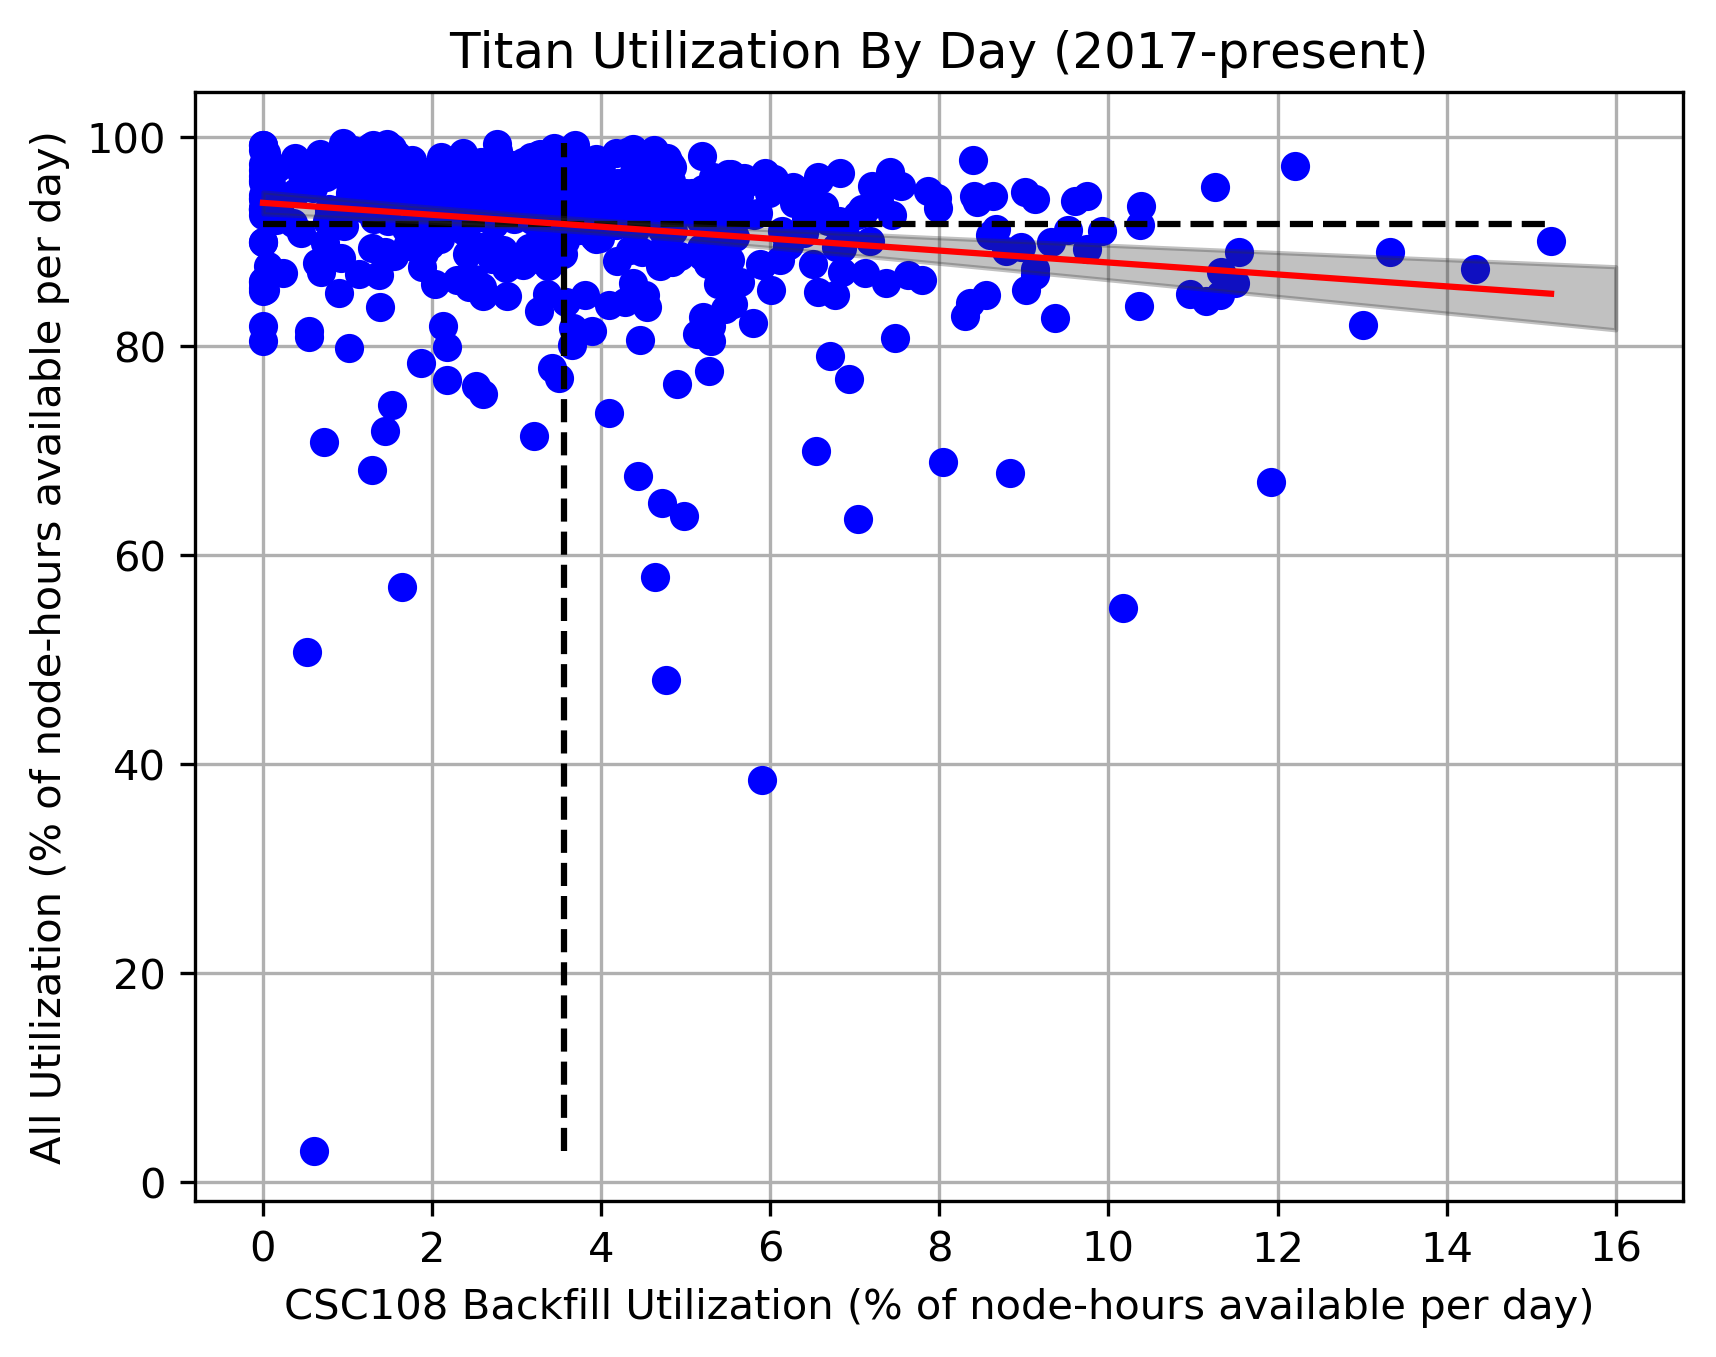
\includegraphics[width=0.75\textwidth]{images/linfit-utilization-by-true-day-all.png}
% figure caption is below the figure
\caption{Parameters for the model are shown in
    Table~\ref{tab:utilization-params}.}
\label{fig:utilization-all}
\end{figure*}


% For two-column wide figures use
\begin{figure*}
% Use the relevant command to insert your figure file.
% For example, with the graphicx package use
  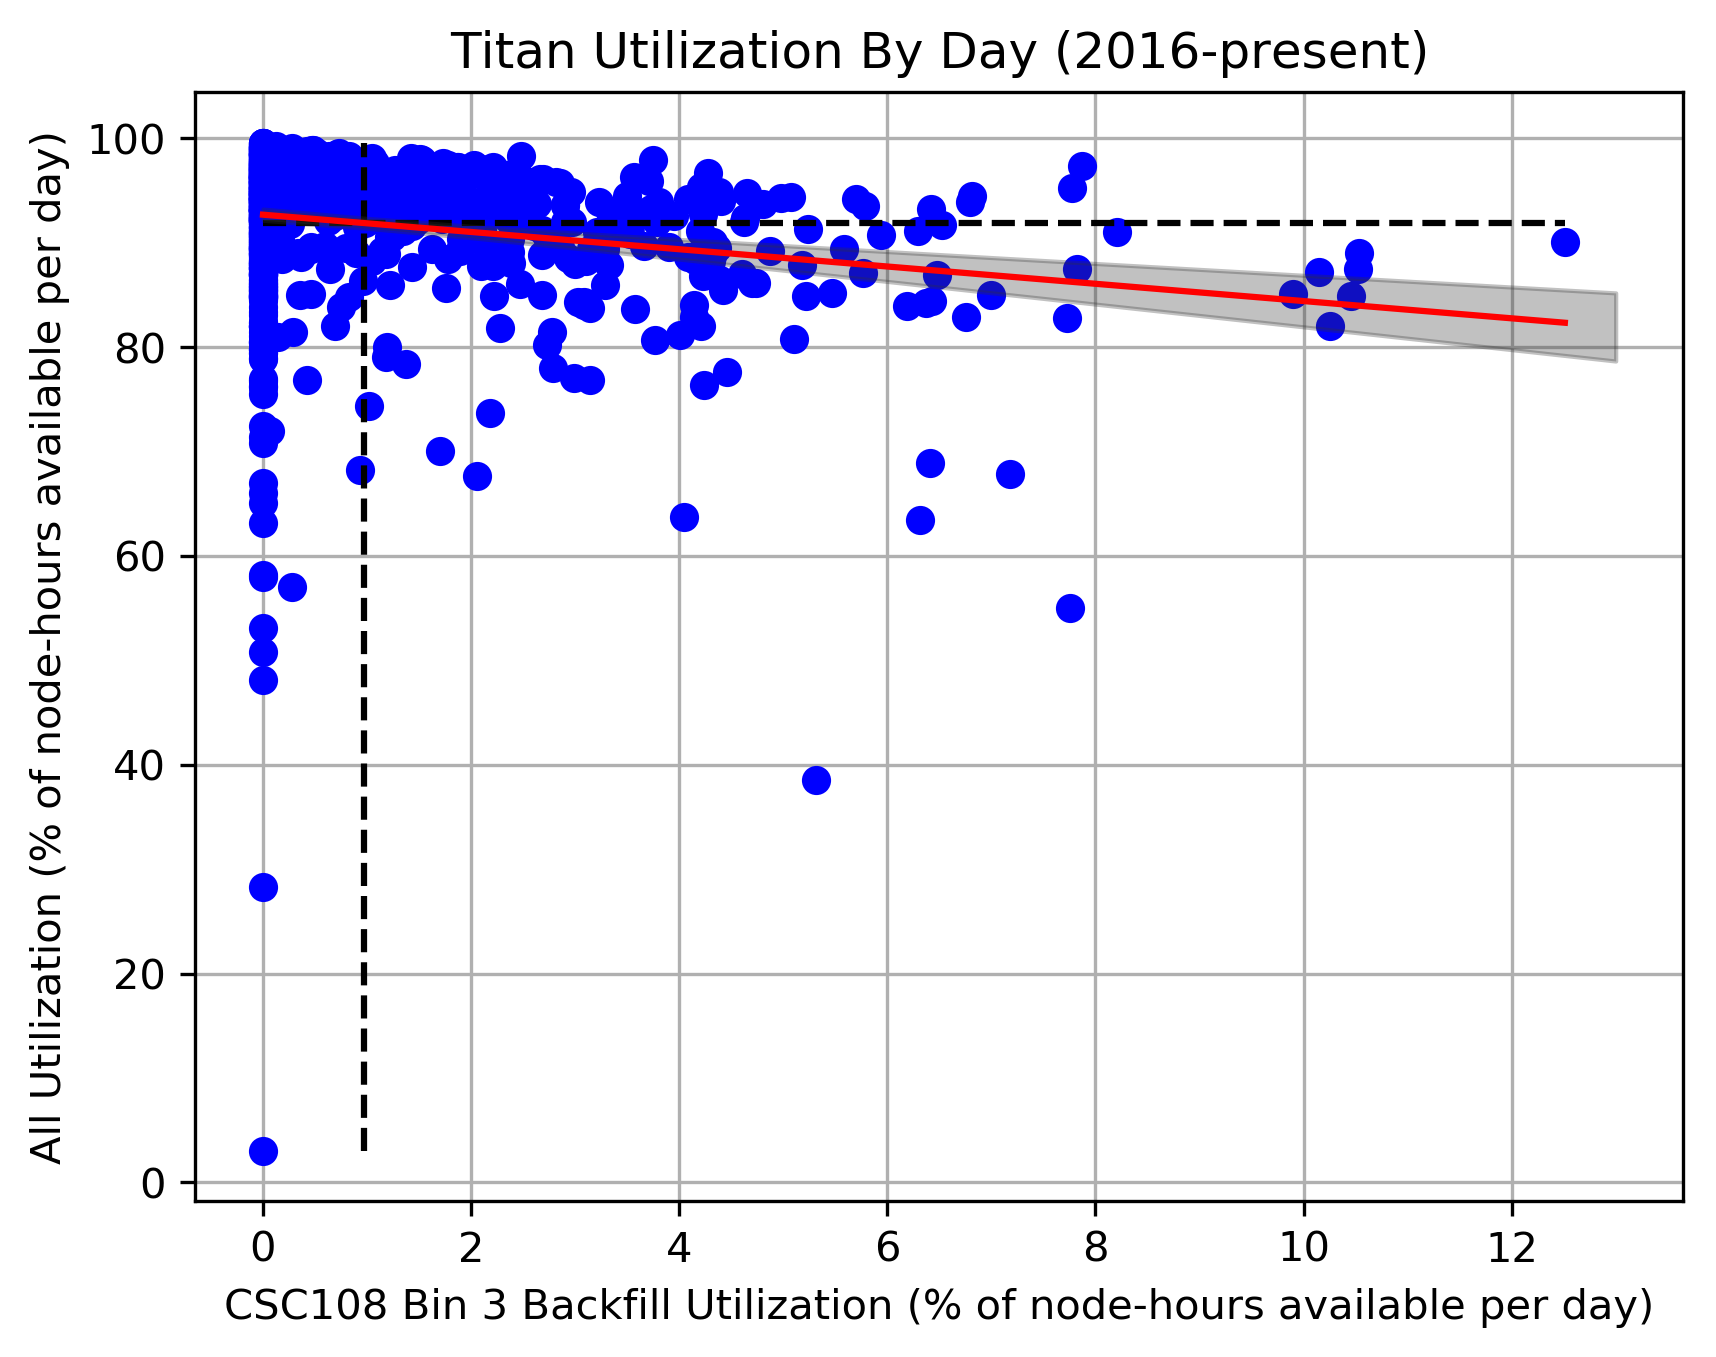
\includegraphics[width=0.75\textwidth]{images/linfit-utilization-by-true-day-bin3.png}
% figure caption is below the figure
\caption{Parameters for the model are shown in
    Table~\ref{tab:utilization-params}.}
\label{fig:utilization-bin3}
\end{figure*}


% For two-column wide figures use
\begin{figure*}
% Use the relevant command to insert your figure file.
% For example, with the graphicx package use
  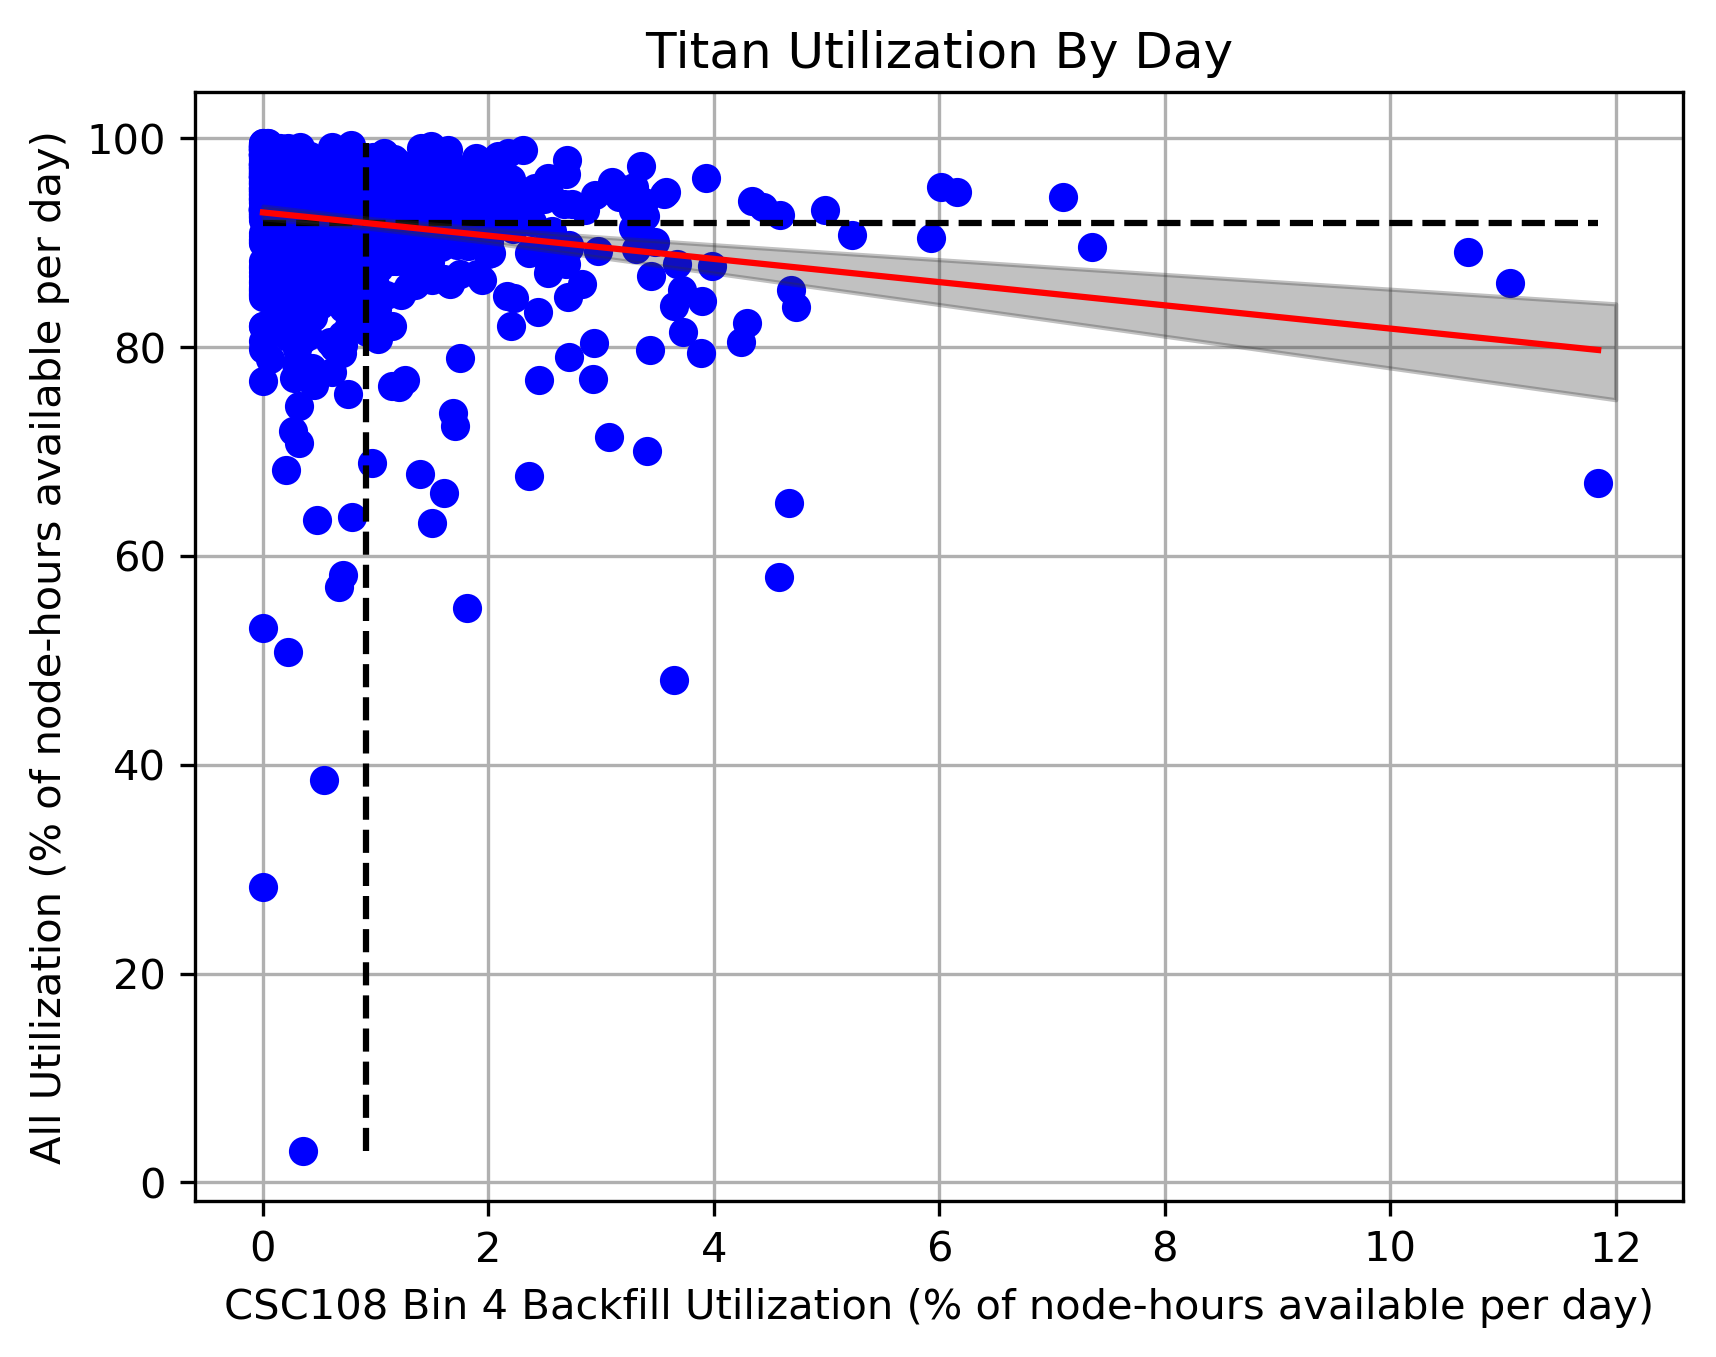
\includegraphics[width=0.75\textwidth]{images/linfit-utilization-by-true-day-bin4.png}
% figure caption is below the figure
\caption{Parameters for the model are shown in
    Table~\ref{tab:utilization-params}.}
\label{fig:utilization-bin4}
\end{figure*}


% For two-column wide figures use
\begin{figure*}
% Use the relevant command to insert your figure file.
% For example, with the graphicx package use
  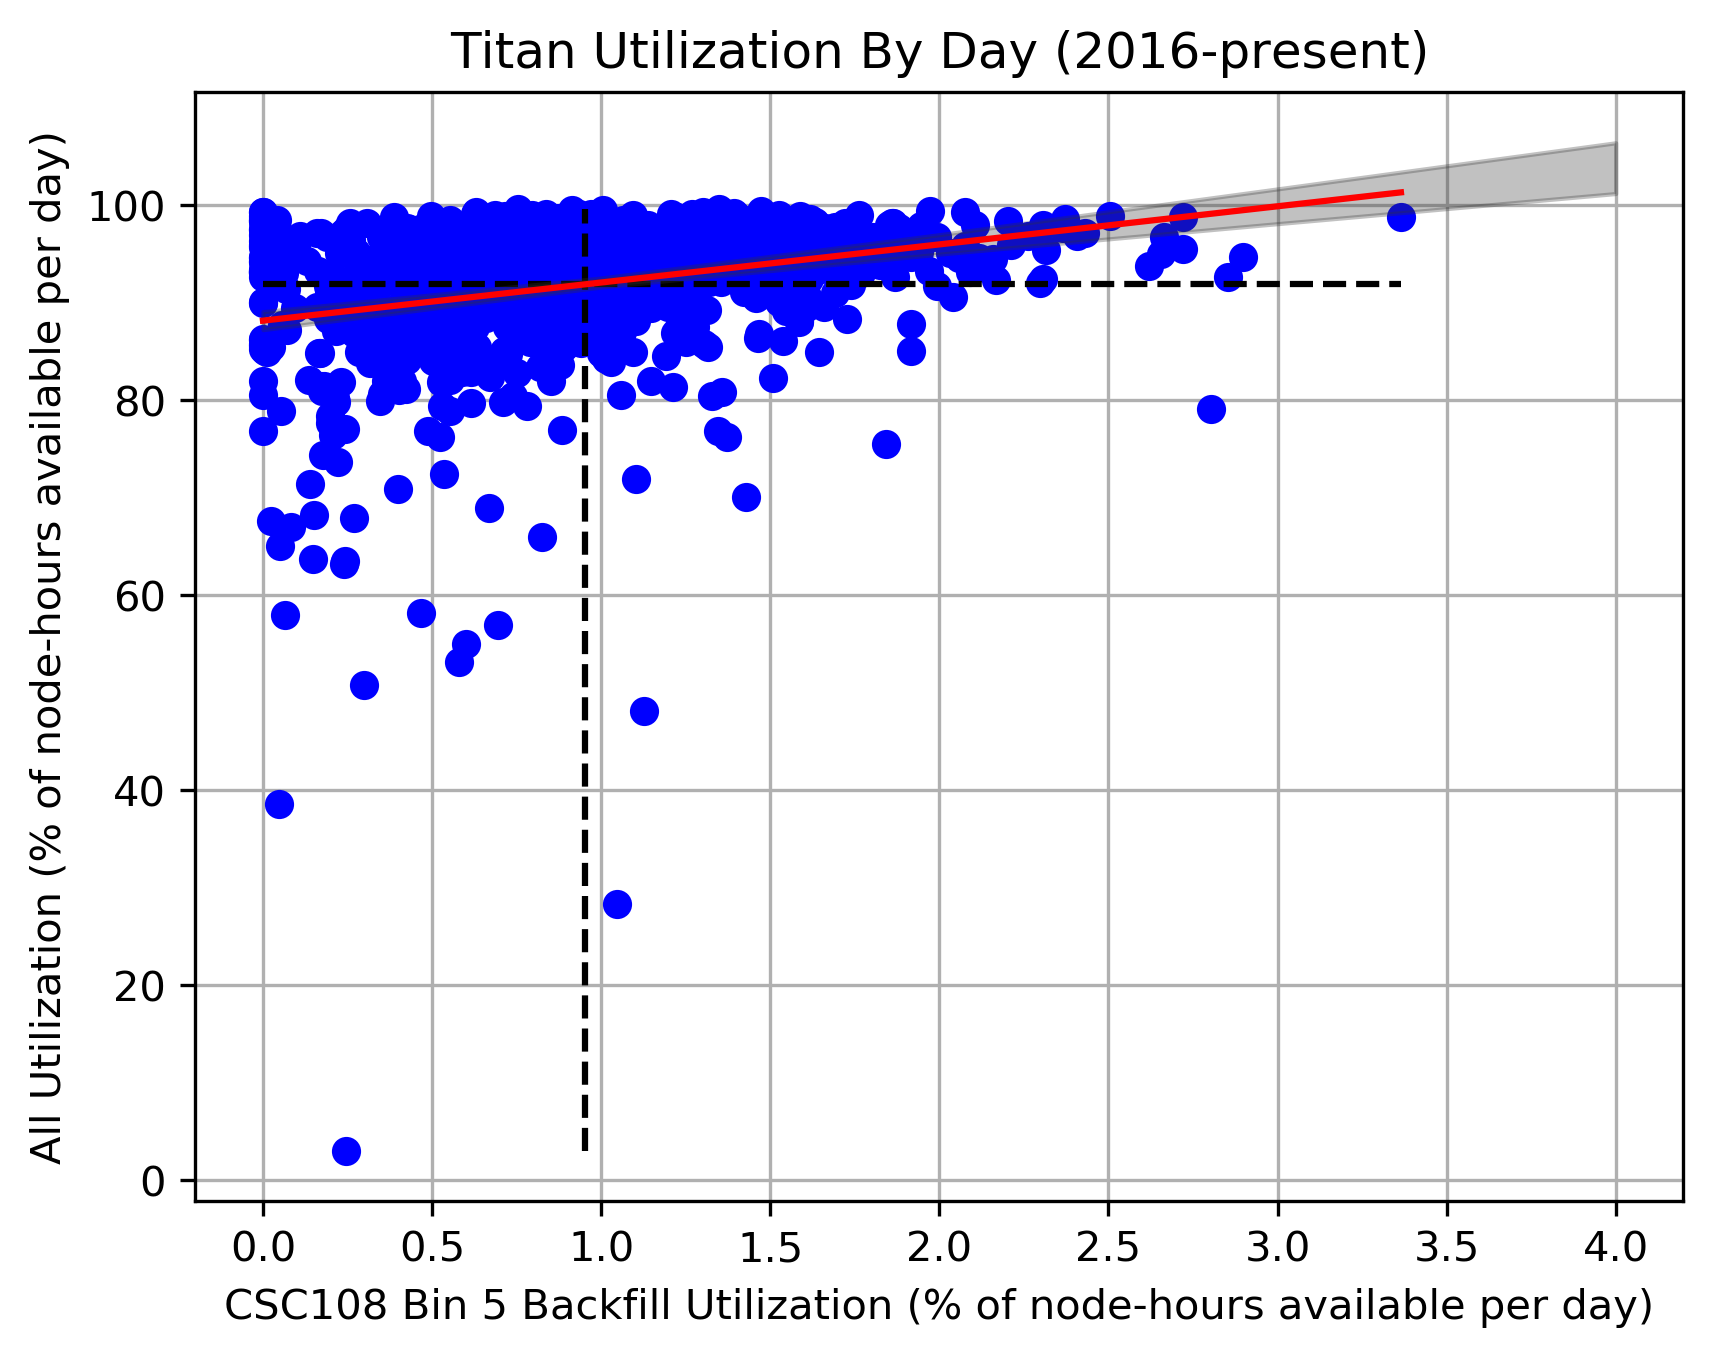
\includegraphics[width=0.75\textwidth]{images/linfit-utilization-by-true-day-bin5.png}
% figure caption is below the figure
\caption{Parameters for the model are shown in
    Table~\ref{tab:utilization-params}.}
\label{fig:utilization-bin5}
\end{figure*}


%%%%%%%%%%%%%%%%%%%%%%%%%%%%%%%%%%%%%%%%%%%%%%%%%%%%%%%%%%%%%%%%%%%%%%%%%%%%%%%%
\subsection{Conclusions}
\label{subsec:sec4-conclusions}

In conclusion,
\begin{itemize}
    \item We probably need to restrict ourselves to being ``sand'' and not
        ``pebbles''
    \item Further results are needed to confirm these trends, and studies are
        ongoing.
\end{itemize}


%-  vim:set syntax=tex:
